\documentclass[11pt,letterpaper]{article}
\usepackage[margin=0.95in]{geometry}
\usepackage{amsmath,amssymb,amsthm,mathtools,booktabs,longtable,array}
\usepackage{microtype,xcolor,graphicx,hyperref}
\hypersetup{colorlinks=true,linkcolor=blue!45!black,urlcolor=blue!45!black,
 pdftitle={QI--Radon construction: networks, error bounds, and allocation}}
\setlength{\parindent}{0pt}
\setlength{\parskip}{5pt}
\setlength{\emergencystretch}{2em}
\allowdisplaybreaks
\setlength{\textfloatsep}{12pt plus 2pt minus 2pt}
\setlength{\intextsep}{12pt plus 2pt minus 2pt}
\renewcommand{\topfraction}{0.85}
\renewcommand{\bottomfraction}{0.6}
\renewcommand{\textfraction}{0.12}
\newcommand{\R}{\mathbb R}
\newcommand{\C}{\mathbb C}
\newcommand{\N}{\mathbb N}
\newcommand{\Z}{\mathbb Z}
\newcommand{\dd}{\,\mathrm d}
\newcommand{\ii}{\mathrm i}
\newcommand{\eps}{\varepsilon}
\newcommand{\norm}[1]{\left\lVert#1\right\rVert}
\newcommand{\abs}[1]{\left|#1\right|}
\newcommand{\Sph}{\mathbb S^{d-1}}
\newcommand{\Ball}{\overline B_1(0)}
\newcommand{\HH}{\mathcal H}
\newcommand{\ord}{\operatorname{ord}}
\newcommand{\GELU}{\operatorname{GELU}}
\newcommand{\ReLU}{\operatorname{ReLU}}
\newcommand{\lean}[1]{\par\smallskip{\footnotesize\textsf{Lean source: }\path{#1}}\par}
\newtheorem{theorem}{Theorem}
\newtheorem{lemma}{Lemma}[section]
\newtheorem{corollary}[lemma]{Corollary}
\theoremstyle{definition}
\newtheorem{definition}[lemma]{Definition}
\theoremstyle{remark}
\newtheorem*{remark}{Remark}
\title{QI--Radon construction\\[4pt]
\large Finite shallow networks, approximation bounds, and resolution allocation}
\author{}
\date{October 9, 2026}
\begin{document}
\maketitle
\vspace{-1em}
\section*{TL;DR}
This note constructs an ordinary one-hidden-layer neural network from a
\textbf{known function by calculating its weights}. Radon decomposition
reduces the function to one-dimensional profiles along different directions.
QI constructs those profiles, and their weighted sum reconstructs the target.
No training or least-squares readout fit is required.

\begin{itemize}
\item \textbf{Analytic functions admit a logarithmic width bound.}
For Gaussian, erf, GELU, and corrected tanh, the sufficient neuron count is
\(W=O(\log^d(1/\eps))\) under the stated assumptions, where \(d\) is input
dimension and \(\eps\) is the requested error. In plain terms, the bound grows
like the number of requested accurate digits raised to the dimension.
All halo neurons are counted; the constants depend on the function and dimension.

\item \textbf{Finite smoothness gives slower, algebraic rates.}
The bounds separate variation along and between directions.
Activation choice matters: ReLU has only an algebraic rate even
for the simple quadratic \(x^2\).

\item \textbf{Directions and centers have a computable allocation rule.}
Their separate error rates determine how to divide resolution. The rule
minimizes the stated sufficient width bound, rather than claiming the best
possible network.

\item \textbf{Boundaries and numerical accuracy are part of the argument.}
The finite-halo correction is included in the construction and proof.
Separate error budgets specify how accurately the parameters and network
must be evaluated.

\item \textbf{The construction is tested through four dimensions.}
The tested analytic families reach relative sampled errors around \(10^{-14}\).
Separate figures examine dimension scaling and robustness across targets;
additional tests check algebraic rates and resolution allocation.
\end{itemize}

\textbf{Lean verification.} The accompanying library verifies the general
kernel construction, angular bounds, allocation, and numerical perturbation
results. The corrected tanh contour argument and its stronger width
consequences are proved in this note but \textbf{are not yet formalized in Lean}.

These are approximation and neuron-count guarantees for known functions.
Computing their Radon profiles can still be expensive; an unknown PDE solution
requires a separate solving method.

\newpage
\setcounter{tocdepth}{2}
\begingroup\small\setlength{\parskip}{0pt}
\tableofcontents
\endgroup
\newpage

\section{The one-dimensional QI idea}
Quasi-interpolation (QI) prescribes coefficients in a chosen family of translated
features. A derivative describes the change accumulated to recover a function.
If \(g\) is absolutely continuous on \([a,b]\), the fundamental
theorem of calculus can be written
\[
 g(s)=g(a)+\int_a^b g'(c)\,\mathbf 1_{\{c\le s\}}\dd c,
 \qquad a\le s\le b.
\]
Thus a superposition of translated steps, with density \(g'\), recovers \(g\).
A smooth activation replaces the sharp step by a smooth transition. Its
derivative replaces the point mass at the transition by a spread-out kernel.

For a general activation, choose an integer \(r\ge0\), a real nonzero constant
\(\zeta\), and a kernel \(K\) such that
\begin{equation}\label{eq:derivative-kernel}
 \phi^{(r)}(s)=\zeta K(s).
\end{equation}
Write \(K_\gamma(s)=\gamma K(\gamma s)\), where \(\gamma>0\).
Differentiating a translated activation \(r\) times gives
\[
 \frac{\dd^r}{\dd s^r}\phi(\gamma(s-c))
   =\zeta\gamma^rK(\gamma(s-c))
   =\zeta\gamma^{r-1}K_\gamma(s-c).
\]
Consequently, a coefficient density \(\rho\) with
\[
 \rho*K_\gamma=g^{(r)}
\]
produces the desired derivative after the corresponding activation integral
is scaled by \(\gamma/(\zeta\gamma^r)\). The remaining difference from \(g\) is a
polynomial of degree below \(r\), fixed by derivative values at a reference point.

This explains the derivative-shaped readouts in a regular geometry.
If \(K\) has integral one, \(\gamma\) is large enough for the kernel to be
narrow relative to the target variation, and sampling errors are small,
then \(\rho(c)\) is close to \(g^{(r)}(c)\). On a grid \(c_j=jh\), the leading
readout is therefore
\begin{equation}\label{eq:qi-intuition}
 v_j\approx \frac{h\gamma}{\zeta\gamma^r}g^{(r)}(c_j).
\end{equation}
For \(\tanh\), \(r=1\) and \(\zeta=2\) with \(K=\tfrac12\operatorname{sech}^2\);
this is \(v_j\approx \tfrac h2g'(c_j)\).
For GELU, \(r=2\), so the analogous quantity is the second derivative.
For a raw normalized bump, \(r=0\), it is the function itself.

Equation \eqref{eq:qi-intuition} is an interpretation, not the finite-accuracy
theorem. Overlapping kernels smooth their coefficient density. The construction
below compensates for that smoothing by deconvolution, and separately controls
the errors from frequency truncation, discrete centers, and finite halos.

\section{Why Radon profiles reduce the problem to spokes}
Throughout the note, Fourier transforms use cycles frequency:
\[
 \widehat F(\xi)=\int_{\R^d}F(x)e^{-2\pi\ii\,\xi\cdot x}\dd x,
 \qquad
 F(x)=\int_{\R^d}\widehat F(\xi)e^{2\pi\ii\,\xi\cdot x}\dd\xi.
\]
For now let \(F\) be a real Schwartz function: it and all its derivatives
decay faster than every power. This makes the integrations and rearrangements
below legitimate. Appendix~\ref{sec:source} constructs such an extension of a
target known only on a bounded region.

Let \(\sigma\) be probability surface measure on \(\Sph\), and let
\[
 s_d=\frac{2\pi^{d/2}}{\Gamma(d/2)}
\]
be the ordinary surface area of the sphere. Polar coordinates in frequency
space give
\[
 F(x)=s_d\int_{\Sph}\int_0^\infty
       \widehat F(t\theta)e^{2\pi\ii t\,\theta\cdot x}t^{d-1}\dd t\,\dd\sigma(\theta).
\]
Pairing the directions \(\theta\) and \(-\theta\) turns the positive radial
integral into half of an integral over the real line. Define the scalar profile
\begin{equation}\label{eq:profile}
 g_\theta(s)=\frac{s_d}{2}\int_\R
       |t|^{d-1}\widehat F(t\theta)e^{2\pi\ii ts}\dd t.
\end{equation}
For real \(F\), this profile is real on real \(s\), and
\begin{equation}\label{eq:radon-reconstruction}
 F(x)=\int_{\Sph}g_\theta(\theta\cdot x)\dd\sigma(\theta),
 \qquad g_{-\theta}(-s)=g_\theta(s).
\end{equation}

The Radon transform gives a spatial description of the same profile.
For a unit vector \(\theta\), set
\[
 p_\theta(s)=\int_{\theta^\perp}F(s\theta+y)\dd y.
\]
Taking the one-dimensional Fourier transform in \(s\), then using the
orthogonal coordinates \(x=s\theta+y\), gives
\[
 \widehat p_\theta(t)
 =\int_\R\int_{\theta^\perp}F(s\theta+y)e^{-2\pi\ii ts}\dd y\,\dd s
 =\widehat F(t\theta).
\]
This is the Fourier-slice identity. Thus \(g_\theta\) is the Radon projection
filtered by the multiplier \(|t|^{d-1}\), with the factor \(s_d/2\).

Put \(\ell=d-1\). If \(\ell=2k\), filtering is ordinary differentiation:
\[
 g_\theta=\frac{s_d}{2}\frac{(-1)^k}{(2\pi)^\ell}\,p_\theta^{(\ell)}.
\]
If \(\ell=2k+1\), it is differentiation after a Hilbert transform:
\[
 g_\theta=\frac{s_d}{2}\frac{(-1)^k}{(2\pi)^\ell}
       (\HH p_\theta)^{(\ell)},\qquad
 \HH p(s)=\frac1\pi\,\operatorname{PV}\int_\R\frac{p(t)}{s-t}\dd t.
\]
Indeed, the Hilbert multiplier is \(-\ii\operatorname{sign}(t)\); multiplying
it by the odd derivative multiplier produces \(|t|^\ell\) with exactly the
constant displayed above.

A profile is therefore a \emph{filtered hyperplane integral}, not the restriction
\(s\mapsto F(s\theta)\). Each profile contains information from the entire
target. The construction approximates these one-dimensional profiles and
averages them over directions.
\lean{QIRadon/Radon/Reconstruction.lean}


\section{Main theorems and their interpretation}\label{sec:main-results}
Let \(d\ge2\) be the input dimension, \(q\) the angular quadrature order,
\(M=q^{d-1}\) the number of directions, and \(n\) the scalar construction
order. Let \(N\) be the actual number of neurons per direction, including
halos; generally \(n\ne N\). The grid width is \(W_{\rm grid}=MN\).
Any neurons needed for an integration polynomial are counted separately.
The one-dimensional case uses the scalar lemmas directly, with no angular error.
All approximation norms in the theorems are uniform absolute errors on the
closed unit ball. Dimension and regularity constants are held fixed when
writing a big-\(O\) law.

The general activation assumptions used for the rates are:
\begin{description}
\item[(K1)] \(r\in\N\), \(\phi\in C^r(\R)\), \(\zeta\ne0\), and a real Schwartz
kernel \(K\) satisfying \(\phi^{(r)}=\zeta K\).
\item[(K2)] \(\nu>0\), \(c_K,C_K,a_K>0\), \(A_K\ge0\), and, for every \(\xi\in\R\),
\[
 c_Ke^{-A_K|\xi|^\nu}\le|\widehat K(\xi)|
       \le C_Ke^{-a_K|\xi|^\nu}.
\]
\item[(K3)] \(\mu>0\), \(C_s,b_K>0\), and, for every \(t\in\R\),
\[
 |K(t)|\le C_se^{-b_K|t|^\mu}.
\]
\end{description}
In particular the transform never vanishes. \(K\) need not be nonnegative.
These are sufficient conditions for this construction; they are not claimed
necessary for neural approximation in general.


The generic spectral construction has scalar count exponent
\(\kappa_{\rm gen}=\max\{1,1/\nu+1/\mu\}\). The first kernel exponent
describes spectral decay; the second describes spatial tails. The corrected
tanh construction improves its scalar count to linear. In the main results use
\[
 \kappa=\begin{cases}1,&\text{tanh with the finite-halo correction},\\
 \kappa_{\rm gen},&\text{the general spectral construction}.
 \end{cases}
\]
Thus Gaussian, erf, GELU, and corrected tanh all have \(\kappa=1\).
The corrected tanh rate requires the finite-halo correction.

\subsection{Analytic functions need only logarithmic resolution}
\begin{theorem}[Analytic targets: geometric error and logarithmic width]\label{thm:main}
Let \(d\ge2\). Assume \(f\) is real on the real ball of radius \(R>1\),
and extends holomorphically to the complex \(\sigma_0\)-neighborhood of that
ball, with \(|f|\le B_f\) there, where \(\sigma_0>0\) and \(B_f\ge0\).
Assume the activation conditions (K1)--(K3). Use the fixed boundary
extension in Section~\ref{sec:construction}, fix \(T_0>1\), and choose
\(H,Z\) by \eqref{eq:HZ}.
Use the profile constants \(\delta,M_g,a,A_\theta\) supplied in
Appendix~\ref{sec:source}. Put
\(U=A_\theta\sqrt{(1+e^{-a})/(1-e^{-a})^{d-1}}\) and
\(b=b_{\rm sc}\) from \eqref{eq:scalar-rate}.
For the general spectral construction take \(V\) from \eqref{eq:V},
\(C=C_{\rm grid}\), and \(\kappa=\kappa_{\rm gen}\).
For corrected tanh take \(V=V_{\tanh}\), \(C=C_{\tanh}\), and \(\kappa=1\)
from Lemma~\ref{lem:tanh-prepared}. All these constants depend only on the
stated target, activation, and fixed construction margins.
For every pair of positive integers \(q,n\), the finite construction obeys
\begin{equation}\label{eq:main-finite}
 \norm{\widehat f-f}_{L^\infty(\Ball)}
       \le Ue^{-aq}+2Ve^{-bn},\qquad
 W_{\rm grid}\le Cq^{d-1}n^\kappa .
\end{equation}
For every requested \(\eps>0\), the explicit order rule
\eqref{eq:orders} gives error at most \(\eps\), and
\begin{equation}\label{eq:geometric-width}
 W_{\rm grid}=O\!\left(\log^{d-1+\kappa}(1/\eps)\right).
\end{equation}
For \(r\le1\) this is an ordinary shallow MLP with exactly the grid index set.
For general \(r\), this statement concerns the grid plus its explicit
integration polynomial until an anchor representation is supplied.
\end{theorem}
\textbf{Interpretation.} The scalar and angular errors add, with no factor
equal to the number of directions. A fixed increase in each resolution
reduces the bound by a fixed factor. Gaussian, erf, and standard
GELU have \(\mu=\nu=2\), hence \(\kappa=1\) and total width
\(O(\log^d(1/\eps))\). GELU needs two additional neurons for its anchor.
The constants depend on the target's frequency content, analytic margins,
activation properties, and dimension.

For tanh, the generic estimates give an extra logarithmic factor.
The finite-halo correction removes it, giving the same \(\log^d(1/\eps)\)
width law. Section~\ref{sec:corrected-tanh} proves this correction;
Lean currently verifies only the generic tanh bound.

\subsection{Finite smoothness gives an algebraic law}
\begin{theorem}[Finite smoothness: algebraic error and width]\label{thm:multi-algebraic}
For real profiles \(g_\theta\), define
\(H_x(\theta)=g_\theta(\theta\cdot x)-g_\theta(0)\).
Let a target on \(\Ball\) satisfy
\[
 f(x)=f(0)+\int_{\Sph}H_x(\theta)\dd\sigma(\theta)
 \quad(\norm{x}\le1).
\]
Assume:
\begin{enumerate}
\item (K1)--(K3), fixed \(T_0>1\), and the prescribed \(H,Z\) inequalities;
\item uniformly in \(\theta\), \(|g_\theta|\le B_g\) on \([-1,1]\), and for
      every integer \(n\ge1\) a polynomial of degree below \(n\)
      approximates \(g_\theta\) there with error at most \(A_pn^{-s_0}\),
      with \(A_p,B_g\ge0\), \(s_0>0\);
\item for every \(x\in\Ball\), \(H_x\) is continuous and even, and
\[
 \sum_{\ell\ge0}(1+\ell)^{2s_\theta}
       \norm{(H_x)_\ell}_2^2\le A_\theta^2
 \quad\text{with }s_\theta>(d-1)/2,\ A_\theta\ge0,
\]
      uniformly in \(x\).
\end{enumerate}
Here \((H_x)_\ell\) is the orthogonal projection onto spherical harmonics
of degree \(\ell\), and \(\|\cdot\|_2\) uses probability surface measure.
Set \(t=s_\theta-(d-1)/2\), \(U_{\rm alg}=C_dA_\theta/\sqrt{2t}\).
For the generic spectral recipe use \(V_{\rm alg}\) and \(C_{\rm grid}\)
from Lemma~\ref{thm:algebraic-row}, with \(\kappa=\kappa_{\rm gen}\).
For corrected tanh use \(V_{\rm alg}^{\tanh}\) and \(C_{\tanh}\) from
Lemma~\ref{lem:tanh-prepared}, with \(\kappa=1\).
Below, \(V_{\rm alg}\) and \(C\) denote the selected constants.
The real-sample construction has
\[
 E(q,n)\le U_{\rm alg}q^{-t}+2V_{\rm alg}n^{-s_0},\qquad
 W_{\rm grid}\le Cq^{d-1}(2n)^\kappa .
\]
It attains any \(\eps>0\) with
\begin{equation}\label{eq:algebraic-width}
 W_{\rm grid}=O\!\left(
    \eps^{-[(d-1)/t+\kappa/s_0]}\right).
\end{equation}
For the separate global Fourier-moment scalar class of
Lemma~\ref{thm:global-algebraic}, with a common moment bound and the same
angular assumptions, the exponent is instead \((d-1)/t+1/s_0\).
Ordinary-MLP conclusions retain the anchor conditions of
Lemma~\ref{thm:anchor}.
\end{theorem}
\textbf{Interpretation.} Angular roughness and scalar roughness are distinct
costs. Their reciprocal smoothness exponents add when directions and centers
are multiplied. This theorem requires the displayed quantitative profile
assumptions. It does not say that every nonanalytic function has the same
rate, nor does the library yet derive these assumptions from general
\(C^s\) target bounds. ReLU is covered by a separate algebraic corollary:
even for \(x^2\), its best possible order is \(W^{-2}\), not geometric.

\subsection{The two resolutions should follow their separate error rates}
\begin{theorem}[How to divide resolution between directions and centers]\label{thm:split}
In the algebraic model
\[
 E_\theta=Uq^{-t},\qquad E_{\rm sc}=Vn^{-s_0},\qquad
 \text{cost}=Cq^p n^\kappa,
\]
assume \(U,V,C,t,s_0,p,\kappa,\eps>0\).
Let \(P=p/t\), \(Q=\kappa/s_0\). Ignoring minimum orders and integer rounding,
the unique optimum assigns
\[
 \eps_\theta=\frac{P}{P+Q}\eps,\qquad
 \eps_{\rm sc}=\frac{Q}{P+Q}\eps.
\]

In the analytic model \(E_\theta=Ue^{-aq}\), \(E_{\rm sc}=Ve^{-bn}\),
assume \(U,V,a,b,C,p,\kappa>0\) and
\(0<\eps<\min(U,V)/e\).
The unique optimum has \(\eps_\theta=x\in(0,\eps)\) solving
\begin{equation}\label{eq:balance}
 \kappa x\log(U/x)
   =p(\eps-x)\log(V/(\eps-x)).
\end{equation}
With all constants fixed as \(\eps\downarrow0\),
\[
 \frac{\eps_\theta}{\eps}\longrightarrow\frac{p}{p+\kappa},
 \qquad
 \frac{n}{q}\longrightarrow\frac{a}{b}.
\]
For this construction \(p=d-1\).
\end{theorem}
\textbf{Interpretation.} If scalar profiles are harder to resolve, the scalar
rate \(b\) is smaller and more centers are needed per angular order.
The answer is a one-variable monotone equation, so it is straightforward to
compute by bisection. It minimizes the stated continuous width bound;
integer rounding, minimum orders, and conservative constants affect practical
performance.
For corrected tanh, \(\kappa=1\): asymptotically the angular budget fraction
is \((d-1)/d\) and the scalar fraction is \(1/d\). In one dimension there is no angular
allocation problem.

\subsection{Numerical errors must be controlled as well as width}
\begin{theorem}[How accurate the numerical computation must be]\label{thm:arithmetic}
Consider the exact network
\(Q(x)=b_0+\sum_{i=1}^Wv_i\phi(a_i\cdot x+b_i)\)
at an input with \(|x_k|\le R_x\), \(R_x\ge0\).
Suppose \(B_\phi,L_\phi,S_v\ge0\) satisfy
\[
 \sum_i|v_i|\le S_v,\qquad
 |\phi(a_i\cdot x+b_i)|\le B_\phi,
\]
and the activation is \(L_\phi\)-Lipschitz between each exact and rounded
preactivation. Let \(0\le\eta\le1\).
Assume every incoming weight, hidden bias, readout, and output bias is perturbed
by at most \(\eta\); each activation evaluation has absolute error at most
\(\eta\); and the final summation has absolute error at most \(\eta\).
Then the computed output \(Q_{\rm num}(x)\) satisfies
\begin{align}
 |Q_{\rm num}(x)-Q(x)|&\le C_{\rm arith}\eta,\label{eq:arith}\\
 C_{\rm arith}&=2+B_\phi W+
        (S_v+W)\bigl(L_\phi(dR_x+1)+1\bigr).\nonumber
\end{align}
Thus absolute tolerance \(\eta=2^{-b_{\rm work}}\) is sufficient for budget
\(\eps_{\rm arith}>0\) if
\[
 b_{\rm work}=
 \left\lceil\max\{0,\log_2(C_{\rm arith}/\eps_{\rm arith})\}\right\rceil.
\]
\end{theorem}
\textbf{Interpretation.} More neurons only improve the exact-arithmetic
approximation. Coefficient magnitudes and the accuracy of the numerical
operations determine the attainable floor. The theorem gives explicit
absolute tolerances; it does not claim that a chosen machine format
satisfies those tolerances automatically.

\section{The construction: from a known function to network weights}\label{sec:construction}
The steps below specify the network parameters. The proofs are in
Section~\ref{sec:theorems}.
The domain is the Euclidean closed unit ball in dimension \(d\ge2\).
The scalar construction itself also applies independently in one dimension.


\subsection{Implementation algorithm}
The inputs are a known real target on a neighborhood of the unit ball, its
analytic or finite-smooth regularity bounds, an activation satisfying the
relevant theorem, and an error tolerance. An implementation must be able to
evaluate the indicated finite integrals to a specified absolute accuracy.
\begin{enumerate}
\item \textbf{Choose the extension.} If a suitable global target is already
available, use it. Otherwise form the smooth real cutoff below, keeping it
identically one on the required domain. This fixes which Radon profiles will
be constructed; it does not change the target on the domain.
\item \textbf{Choose the two resolutions.} Reserve part of the error for
numerical evaluation. Use Theorem~\ref{thm:split} to allocate the rest between
angular order \(q\) and scalar order \(n\), then round both upward. The
half-and-half choice \eqref{eq:orders} is a simpler sufficient alternative.
\item \textbf{Generate directions and weights.} Construct the recursive
Gauss--Jacobi rule below, fold antipodal pairs, and retain
\((\theta_m,\alpha_m)\), \(m=1,\ldots,M=q^{d-1}\).
The weights are positive and sum to one.
\item \textbf{Compute each filtered Radon profile.} Integrate over the
hyperplanes normal to \(\theta_m\), then apply the derivative/Hilbert filter
in Section~2, or use a justified Fourier formula for the same profile.
The profile is not the restriction \(f(s\theta_m)\).
\item \textbf{Compute scalar readouts.} For the general verified construction,
apply the cosine-transform sample polynomial and window below, compute its
Fourier transform, divide the derivative spectrum by
\(\widehat K(\xi/\gamma)\) on \([-B,B]\), and evaluate \eqref{eq:density}
at the retained centers. The formulas below specify \(\gamma,h,B\) and the
full halo. For tanh, use the corrected geometry in
Section~\ref{sec:corrected-tanh}, or Lemma~\ref{lem:tanh-prepared} when
preparation is needed, and the readouts in Corollary~\ref{cor:tanh-shift}.
Section~\ref{sec:lambda-choice} gives an optional lambda sweep; recompute
the error bound for each changed geometry. If the original
profile already has a known complex neighborhood, apply the same formula
directly to that profile and omit the preparation polynomial.
\item \textbf{Set the integration constants and flatten the network.}
Apply the derivative anchors below. Multiply each scalar readout by
\(\alpha_m\), use incoming vector \(\gamma\theta_m\) and hidden bias
\(-\gamma c_j\), and choose the output constant so the result equals \(f(0)\).
For GELU, absorb the combined linear anchor into two additional GELU neurons.
A higher-order activation needs its own anchor representation.
\item \textbf{Check numerical accuracy.} Budget profile, quadrature, coefficient,
and evaluation errors using Theorem~\ref{thm:arithmetic}. Refining a numerical
integral is a useful diagnostic; agreement alone is not a rigorous error
certificate. Count every halo and anchor neuron in the reported width.
\end{enumerate}
No least-squares fit occurs in these steps. The work required to obtain the
profiles may still be substantial; the width theorem is not a runtime theorem.

\subsection{The input and the boundary extension}\label{sec:target-input}
The analytic input consists of \(f:\R^d\to\R\), constants \(R>1\),
\(\sigma_0>0\), \(B_f\ge0\), and a holomorphic function
\(\mathcal F:\C^d\to\C\) on the tube
\[
 \mathcal T(R,\sigma_0)
 =\{z:\text{there exists }x\in\R^d,\ \norm{x}\le R,\
                      \norm{z-x}<\sigma_0\}.
\]
Here real vectors are embedded in \(\C^d\), both with their Euclidean norms.
Require \(|\mathcal F(z)|\le B_f\) throughout this tube and
\(\mathcal F(x)=f(x)\) for every real \(\norm{x}\le R\).

Choose the prescribed margins in Section~\ref{sec:source}, including
\(1<R_0<R\). Define
\[
 w(a)=
 \frac{\mathbf 1_{\{R_0<a<R\}}
       \exp(-1/[(a-R_0)(R-a)])}
      {\int_{R_0}^{R}\exp(-1/[(u-R_0)(R-u)])\dd u},
 \qquad
 \chi(r)=\int_{R_0}^{R}w(a)\mathbf 1_{\{r\le a\}}\dd a .
\]
The extension \(F(x)=f(x)\chi(\norm{x})\) on the outer ball, and zero outside,
is smooth, compactly supported, and exactly equal to \(f\) on the unit ball.
The cutoff is smooth, not globally analytic; only the target's local
analyticity is used.

Compute the profiles \eqref{eq:profile} of this extension, or equivalently use
the finite Radon and regularized Hilbert formulas in
Section~\ref{sec:source}. The latter provide the local complex continuation.
Substituting complex arguments into the full Fourier integral without a
convergence justification would not be valid.

\subsection{The direction grid and its weights}
Let \(q\ge1\) be the angular quadrature order. On the circle use \(2q\)
equally spaced angles, with weight \(1/(2q)\). In dimension \(d\ge3\), write
\[
 \theta=(\sqrt{1-t^2}\,\omega,t),\qquad \omega\in\mathbb S^{d-2},
\]
and apply \(q\)-point Gauss--Jacobi quadrature in \(t\) with probability weight
\[
 \frac{(1-t^2)^{(d-3)/2}}{Z_d},\qquad
 Z_d=\int_{-1}^{1}(1-t^2)^{(d-3)/2}\dd t
     =\frac{\sqrt\pi\,\Gamma((d-1)/2)}{\Gamma(d/2)}.
\]
Repeat this recursively for \(\omega\).

The \(q\) nodes are the roots of the degree-\(q\)
orthogonal polynomial for the displayed positive weight. If \(L_j\) is the
Lagrange cardinal polynomial of node \(j\), its normalized Gaussian weight is
\(\int_{-1}^1L_j(t)^2(1-t^2)^{(d-3)/2}\dd t/Z_d\).
These are finite one-dimensional polynomial integrals. Multiply the weights
across the recursion. The full rule has \(2q^{d-1}\) nodes.

The centered integrand
\[
 H_x(\theta)=g_\theta(\theta\cdot x)-g_\theta(0)
\]
is even in \(\theta\). Retain one node from each antipodal pair and add the
pair's weights. This leaves
\[
 M=q^{d-1},\qquad \alpha_m>0,\qquad \sum_{m=1}^M\alpha_m=1.
\]
The \(\alpha_m\) are quadrature weights. They are generally not \(1/M\).

\subsection{Prepare each scalar profile from finite samples}
Fix a window scale \(T_0>1\), for example \(T_0=2\), and a preparation order
\(n\ge1\). Evaluate a real profile \(g\) at
\[
 t_j=\cos\frac{(2j+1)\pi}{2(n+1)},\qquad j=0,\ldots,n.
\]
Its sample polynomial is
\[
 P_n(s)=\sum_{k=0}^n a_kT_k(s),\qquad
 a_k=\frac{2-\mathbf 1_{\{k=0\}}}{n+1}
           \sum_{j=0}^ng(t_j)T_k(t_j),
\]
where \(T_k(\cos t)=\cos(kt)\). This is a finite cosine transform, not
least-squares fitting.

Multiply by the entire flat window
\begin{equation}\label{eq:prepared}
 u_n(z)=P_n(z)\,e^{-n(z/T_0)^2}
             \sum_{k=0}^n\frac{[n(z/T_0)^2]^k}{k!}.
\end{equation}
It is close to \(g\) on \([-1,1]\), while decaying along horizontal lines.
Its derivative spectrum is
\[
 \widehat p_n(\xi)=(2\pi\ii\xi)^r\widehat u_n(\xi).
\]
All frequency integrals in the next step concern this explicitly prepared
function. They do not require complex evaluations of the original target
outside its given neighborhood.

\subsection{Prescribe bandwidth, spacing, and halos}\label{sec:bandwidth}
Use the activation constants in (K1)--(K3).

Define
\begin{align}
 H&=2\max\{1,((A_K+4)/a_K)^{1/\nu}\},&
 Z&=(2(A_K+3)/b_K)^{1/\mu},\label{eq:HZ}\\
 G&=\log(2(3+4T_0))+\frac{3}{2T_0^2},&
 L&=(G+3)n,\label{eq:L}\\
 B&=L/\pi,&
 \gamma&=B/L^{1/\nu},\label{eq:bandwidth}\\
 h&=1/(HB),&
 D&=ZL^{1/\mu}/\gamma.\label{eq:halo}
\end{align}
Thus \(H\ge2\), \(A_K+4\le a_K(H/2)^\nu\), and
\(A_K+3\le (b_K/2)Z^\mu\). One may use any fixed \(H,Z\) satisfying these
inequalities instead of \eqref{eq:HZ}.

Retain the finite center set
\[
 J=\{j\in\Z:|j|\le\lfloor(1+D)/h\rfloor\},\qquad c_j=hj.
\]
The part beyond \([-1,1]\) is the halo. Both sides are included in \(J\).
The overlap parameter is \(\lambda=\gamma h=1/(HL^{1/\nu})\); this schedule
varies with accuracy. Here \(n\) is the preparation order, while \(|J|\)
counts all retained centers.

\subsection{Choosing lambda in practice}\label{sec:lambda-choice}
\textbf{Start from the kernel Fourier-ratio rule.} At spacing \(h\), the
first grid frequency is \(1/h\). Scaling the kernel by \(\gamma\) makes its
argument \(1/(\gamma h)=1/\lambda\). For tanh use the normalized derivative
\(K(s)=\tfrac12\operatorname{sech}^2s\). The familiar score is
\begin{equation}\label{eq:lambda-kernel-ratio}
 \mathcal A_K(\lambda)
 =\frac{|\mathcal F_{\rm ang}K(2\pi/\lambda)|}{|\mathcal F_{\rm ang}K(0)|}
 =\frac{|\widehat K(1/\lambda)|}{|\widehat K(0)|}
 =\frac{\pi^2/\lambda}{\sinh(\pi^2/\lambda)}.
\end{equation}
Here \(\mathcal F_{\rm ang}\) uses \(e^{-\ii\omega s}\); the hat notation
elsewhere in this note uses \(e^{-2\pi\ii\xi s}\).
Thus the change from \(2\pi/\lambda\) to \(1/\lambda\) is only a frequency
convention. Numerically,
\[
 \mathcal A_K(0.25)=5.6511\times10^{-16},\qquad
 \mathcal A_K(\lambda_A)=2^{-52}\ \Longrightarrow\ \lambda_A=0.24408\ldots.
\]
This explains the useful float64 default \(\lambda\simeq0.25\).
The score measures kernel alias suppression; it is not the total network error.

\textbf{The corrected bound contains exactly this score.}
Let \(n\ge2\) count interval cells, \(h=2/n\), and \(R\ge1\) count halo
centers per side. Use the actual filtered profiles \(g_{\theta_m}\), assumed
real on \([-1-\Delta,1+\Delta]\), holomorphic on its complex
\(\delta\)-neighborhood, and bounded there by \(B_m\), with common positive
margins \(\Delta,\delta\). The pole term from
Section~\ref{sec:corrected-tanh} satisfies
\begin{equation}\label{eq:lambda-ratio-bridge}
 E_{{\rm pole},m}
 \le\frac{64\pi B_m}{\lambda\delta n}e^{-\pi^2/\lambda}
 =\frac{32B_m}{\pi\delta n}(1-e^{-2\pi^2/\lambda})\mathcal A_K(\lambda)
 \le\frac{32B_m}{\pi\delta n}\mathcal A_K(\lambda).
\end{equation}
The equality follows from \(\sinh z=(e^z-e^{-z})/2\).
Thus the Fourier-ratio rule enters the bound with explicit profile-size,
spacing, and anchoring factors. To choose lambda:

\begin{enumerate}
\item \textbf{Choose the alias threshold.} For a float64 starting sweep,
use \(\eta=2^{-52}\). For a certified absolute alias budget
\(\eps_a\), use \(\eta=\eps_a/C_A\) when \(C_A>0\), where
\[
C_A=\frac{64}{\pi\delta n}\sum_m\alpha_mB_m.
\]
If \(C_A=0\), this alias contribution vanishes.
The factor two accounts for origin anchoring. Select the largest
\(\lambda_A\le1\) with \(\mathcal A_K(\lambda_A)\le\eta\), using scalar bisection
when the threshold is attained. Machine epsilon is a convenient starting
threshold; certification requires the complete error budget.

\item \textbf{Check geometry and start near \(\lambda_A\).} Require
\begin{equation}\label{eq:lambda-admissible}
 (R+\tfrac12)h\le\Delta,\qquad
 \lambda\in I:=\left[\max\left\{\frac{4\pi h}{\delta},
                                  \frac{2\log2}{R}\right\},\,1\right].
\end{equation}
These conditions keep the complex shift \(\pi h/(2\lambda)\) within
\(\delta/8\) and the halo inside the known real margin. Start with, for
example, nine logarithmically spaced values in
\(I_0=I\cap[\lambda_A/2,2\lambda_A]\), including \(0.25\) when admissible.
This is a starting range for a finer sweep, not a guaranteed optimum.
If no admissible value meets a prescribed certified alias budget, revise the
geometry; clipping the seed does not certify that budget.

\item \textbf{Include the halo and numerical errors.} At each candidate,
recompute the readouts, halo correction, and output constant. Use
\begin{equation}\label{eq:lambda-score}
 S_m(\lambda)=\frac{B_m}{\delta}\left[
 32e^{-\pi\delta n/4}
 +\frac{64\pi}{\lambda n}e^{-\pi^2/\lambda}
 +\frac{32D_\lambda}{n}e^{-\lambda R^2/4}\right],
 \qquad D_\lambda=\frac\pi{2\lambda}+\frac{4\log2}{\pi}.
\end{equation}
Combine \(E_{\rm angular}+2\sum_m\alpha_mS_m\) with any preparation and
coefficient/evaluation error allowances (Theorem~\ref{thm:arithmetic}).
Since \(\sum_m\alpha_m=1\), the number of directions introduces no extra
multiplicative factor. The kernel ratio stays the same in higher dimensions;
the filtered profiles and angular error change.

\item \textbf{Refine where the computed error is lowest and stable.}
Check independent real points, including endpoints, and repeat promising
candidates with finer contour quadrature and higher precision. Sweep more
densely in those intervals; expand within \(I\) if the best result is at
an edge. These checks guide empirical selection; the bounds certify uniform
accuracy. Increase centers, halo, precision, or directions if the relevant
error contribution prevents the requested accuracy.
\end{enumerate}

\textbf{Where \(2\pi/R\) belongs.} Balancing the two exact-arithmetic factors
\(e^{-\pi^2/\lambda}\) and \(e^{-\lambda R^2/4}\) gives \(\lambda_R=2\pi/R\).
This helps balance halo resources when both contributions matter. It should
not replace the Fourier-ratio starting rule when aliasing is already below
the working accuracy: extra halo nodes alone do not require a smaller lambda.
As the requested threshold \(\eta\to0\), the ratio rule gives
\(\lambda_A\sim\pi^2/\log(1/\eta)\), consistent with the asymptotic
construction schedule.

For other activations, use their own kernel transform and error bounds;
the tanh halo formula does not transfer automatically. The figures below
use their stated fixed schedules, not a benchmark of this sweep selector.

\subsection{The coefficients, anchors, and final MLP}
For every retained direction compute
\begin{equation}\label{eq:density}
 \rho_m(c)=\operatorname{Re}\int_{-B}^{B}
       \frac{\widehat p_{n,m}(\xi)}{\widehat K(\xi/\gamma)}
                       e^{2\pi\ii\xi c}\dd\xi.
\end{equation}
Form the unanchored spoke sum
\[
 R_m(s)=\frac{h\gamma}{\zeta\gamma^r}
             \sum_{j\in J}\rho_m(c_j)\phi(\gamma(s-c_j)).
\]

The integration polynomial is explicit:
\[
 A_m(s)=\sum_{k=0}^{r-1}
       \frac{u_{n,m}^{(k)}(0)-R_m^{(k)}(0)}{k!}s^k,\qquad
 U_m=R_m+A_m.
\]
An empty sum is zero. The final function is
\begin{equation}\label{eq:network}
 \widehat f(x)=f(0)+\sum_{m=1}^{M}\alpha_m
                     [U_m(\theta_m\cdot x)-U_m(0)].
\end{equation}
For each grid neuron the incoming vector, hidden bias, and readout are
\[
 a_{mj}=\gamma\theta_m,\qquad b_{mj}=-\gamma c_j,\qquad
 v_{mj}=\alpha_m\,\frac{h\gamma}{\zeta\gamma^r}\rho_m(c_j).
\]
The origin subtraction contributes one output constant.

For \(r\le1\), the centered anchors vanish, so this is already an ordinary
MLP with \(M|J|\) hidden neurons. For higher \(r\), the combined anchor must be
represented with the selected activation. It cannot be left as a polynomial
evaluated outside the network. Standard GELU has \(r=2\) and
\(\GELU(t)-\GELU(-t)=t\). Its combined affine anchor is therefore represented
by two neurons total. General higher-order activations require the separate
anchor representation bound stated below.

\subsection{Tanh readouts from a complex shift}\label{sec:tanh-readouts}
For tanh, the scalar density can be evaluated directly at complex arguments.
Use \(g_m=g_{\theta_m}\), or the entire prepared profile when preparation
is required. The following is a convenient form of the corrected construction
in Section~\ref{sec:corrected-tanh}.

\begin{corollary}[Complex-shift tanh readouts]\label{cor:tanh-shift}
Assume the profile and geometry conditions in
Section~\ref{sec:lambda-choice}. Let \(\ii^2=-1\),
\(\gamma=\lambda/h\), \(\tau=\pi/(2\gamma)\), and
\(c_j=-1+jh\), \(-R\le j\le n+R\).
The scalar density and the baseline readout at a real center are
\begin{align}
 \rho_m(c)
 &=\frac{g_m(c+\ii\tau)-g_m(c-\ii\tau)}{2\ii\tau}
   =\frac{\operatorname{Im}g_m(c+\ii\tau)}{\tau},\label{eq:tanh-shift-density}\\
 u^{\rm base}_{mj}
 &=\frac h2\rho_m(c_j)
   =\boxed{\frac{\lambda}{\pi}\operatorname{Im}
      g_m\!\left(c_j+\frac{\ii\pi h}{2\lambda}\right)}.
      \label{eq:tanh-shift-weight}
\end{align}
Let \(\Delta u_{mj}\) be the explicit halo correction from
Section~\ref{sec:corrected-tanh}: add \(\kappa^-_{mi}/2\) to the \(i\)-th
outer left halo slot and subtract \(\kappa^+_{mi}/2\) from the corresponding
right slot, for \(1\le i\le\lfloor(R+1)/2\rfloor\); it is zero elsewhere.
Then the final ordinary network is
\begin{align}
 v_{mj}&=\alpha_m(u^{\rm base}_{mj}+\Delta u_{mj}),\nonumber\\
 b_0&=f(0)-\sum_{m,j}v_{mj}\tanh(-\gamma c_j),\nonumber\\
 \widehat f(x)&=b_0+\sum_{m,j}v_{mj}
                  \tanh\!\bigl(\gamma(\theta_m\cdot x-c_j)\bigr).
                  \label{eq:tanh-final-network}
\end{align}
It has \(M(n+1+2R)\) hidden neurons and is anchored at \(f(0)\).
Its error is controlled by the corrected scalar bound, angular assembly,
and any preparation or numerical errors already described above.
\end{corollary}
\begin{proof}
Since \(g_m\) is holomorphic on a conjugation-symmetric neighborhood and real
on its real interval, \(g_m(c-\ii\tau)=\overline{g_m(c+\ii\tau)}\).
This proves \eqref{eq:tanh-shift-density}, and
\(h/(2\tau)=\gamma h/\pi=\lambda/\pi\) proves the readout formula.
The finite-contour argument in Section~\ref{sec:corrected-tanh} supplies
the density and halo correction. Multiplying by the angular weights and
choosing the displayed constant gives \eqref{eq:tanh-final-network} and
the assembly bound \eqref{eq:assembly}.
\end{proof}

The imaginary displacement is \textbf{not a step to send to zero}: its value
\(\pi/(2\gamma)\) compensates for tanh's smoothing. Where full-line Fourier
transforms and contour shifts are justified, this is seen directly from
\[
 \widehat\rho_m(\xi)=\ii\frac{\sinh(2\pi\tau\xi)}{\tau}\widehat g_m(\xi),
 \qquad
 \widehat K_\gamma(\xi)=\frac{2\pi\tau\xi}{\sinh(2\pi\tau\xi)},
 \qquad K_\gamma(s)=\tfrac\gamma2\operatorname{sech}^2(\gamma s).
\]
The transform of \(K_\gamma\) has continuous value one at \(\xi=0\).
Their product is \(2\pi\ii\xi\widehat g_m(\xi)\), the transform of \(g_m'\).
The local finite-contour proof establishes the coefficient rule without
assuming those full-line transforms exist.
The imaginary-part shortcut applies only at real centers. Inside the complex
halo integrals, retain both shifts in \(\rho_m(z)\).

\section{Empirical checks: scaling and robustness}\label{sec:empirical}
Every analytic experiment uses the explicit tanh readouts and the finite-halo
correction proved in Section~\ref{sec:corrected-tanh}. There is no training,
readout fit, or numerical PDE solution. The scaling figure holds the function
family fixed and changes dimension. The separate robustness figure changes
the target while holding the construction rule fixed.

\subsection{Scaling: one family in four dimensions}
Use the same function family in \(d=1,2,3,4\):
\[
 f_d(x)=\exp\!\left(-3\sum_{k=1}^d x_k^2\right).
\]
Its canonical Radon profiles are explicit; their derivation and the unfitted
bounds are in Appendix~\ref{app:empirical-bounds}. The global Gaussian
already decays sufficiently fast, so this benchmark needs no cutoff extension.
It tests discretization and assembly, not the general cost of acquiring Radon
profiles from an arbitrary target.

The direction rule is the full folded Gauss--Jacobi product rule. Vary
\(q=2,3,4,6,8,10,12,16,20,24\), use \(n=\max(32,8q)\) interval cells,
and fix physical halo \(\ell_0=0.5\) and \(\gamma=4\pi\). Then
\[
 R=\lceil n/4\rceil,\qquad N=n+1+2R,\qquad M=q^{d-1},\qquad W=MN=O(q^d).
\]
In \(d=1\), one direction suffices. Here \(n\) counts cells for the direct
tanh formula, rather than the preparation order used in the general proof.
There is no target-dependent tuning of this resolution schedule.

Each construction is evaluated at 160 fixed independent points with radii
spread over the unit ball, plus the origin and both signs of each coordinate
axis. The relative sampled \(L^2\) error is the norm of the residual vector
divided by the norm of the target vector. It is not a certified continuous
norm. The result files also record the largest error on those points.

\begin{figure}[!htb]
\centering
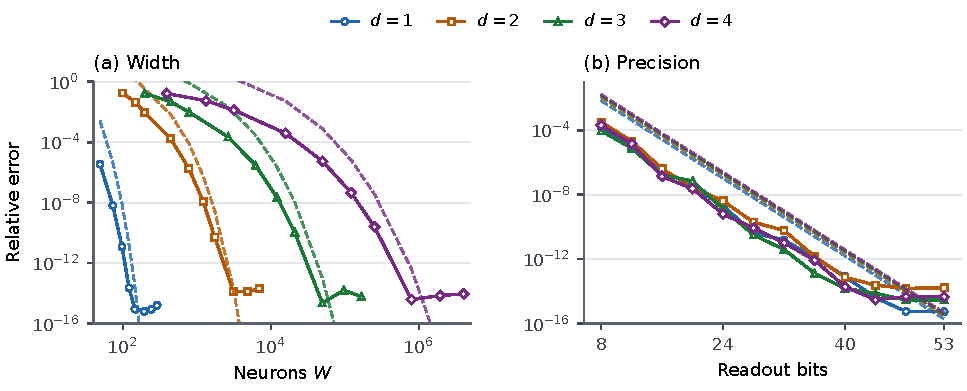
\includegraphics[width=0.97\linewidth]{../empirical/figures/construction_rates.pdf}
\small
\caption{\textbf{Scaling.} The same Gaussian family in four dimensions.
Solid: measured relative $L^2$ error; dashed: corrected bounds, including
readout rounding in (b). Width includes halos. Other operations remain float64.}
\label{fig:main-rates}
\end{figure}

The width bounds combine the explicit angular remainder with the corrected
scalar error. Dividing the uniform absolute bound by sampled target RMS
bounds the plotted relative error in exact arithmetic. The predictions keep
decreasing; the measured errors eventually stop improving because the
calculation uses float64. At the largest tested widths, the relative errors
in dimensions one through four were
\(1.64\times10^{-15}\), \(2.07\times10^{-14}\),
\(6.09\times10^{-15}\), and \(9.31\times10^{-15}\).
The corresponding widths were \(289\), \(6936\), \(166464\), and
\(3{,}995{,}136\). Refinement at this floor is not monotone; all runs are retained.

For the precision panel, fix \(q=20\), \(n=128\), and round only the final
readouts and output bias to \(p=8,12,\ldots,48,53\) significand bits.
The sufficient rounding contribution is
\[
 2^{-p}\left(|b_0|+\sum_j|v_j|\right),
\]
using \(|\tanh|\le1\). The dashed lines add this to the exact-construction
error bound, not to a measured floor. This isolates the readout contribution
to Theorem~\ref{thm:arithmetic}; it is not a \(p\)-bit implementation of the
entire profile, quadrature, and evaluation pipeline.

\subsection{Robustness: vary the target, keep the construction fixed}
Write \(G_{a,c}(x)=e^{-a\|x-c\|^2}\). Let
\(u=(1,\ldots,1)/\sqrt d\), and normalize the vector with coordinates
\(\cos(j+0.7)\), \(j=0,\ldots,d-1\), to obtain \(v\).
The five target families are
\[
 G_{0.5,0},\quad G_{3,0},\quad G_{1.5,0.35u},\quad
 G_{2,-0.35u}+0.7G_{4,0.35v},\quad
 G_{4,-0.45u}-2G_{4,0}+G_{4,0.45u}.
\]
These vary scale, location, number of peaks, and sign under one geometry and
resolution schedule. They test robustness within Gaussian-based analytic
families, rather than across arbitrary function classes.

\begin{figure}[!htb]
\centering
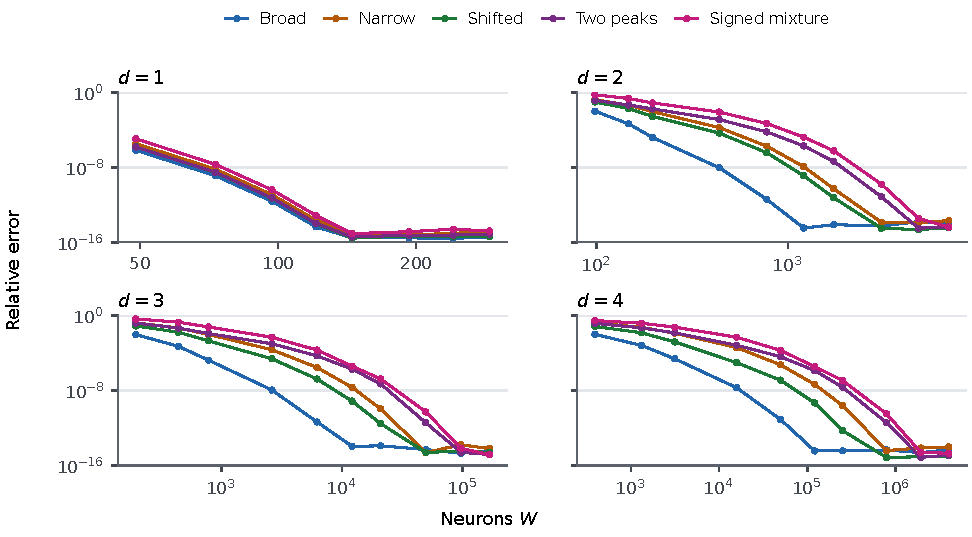
\includegraphics[width=0.97\linewidth]{../empirical/figures/robustness.pdf}
\small
\caption{\textbf{Robustness.} Five Gaussian-based families, using the same
construction and resolution schedule in each dimension. Curves show measured
relative $L^2$ error.}
\label{fig:robustness}
\end{figure}

\subsection{Checks of the other results}
\textbf{Algebraic convergence for a nonanalytic target.} Use the general
spectral construction with Gaussian activation, \(r=0\), and
\[
 \widehat f(\xi)=(1+\xi^2)^{-2},\qquad
 f(x)=\frac\pi2(1+2\pi|x|)e^{-2\pi|x|}.
\]
The target has finite smoothness at zero. Its weighted Fourier moment with
exponent two is exactly \(A_2=\pi+2\). Use the prescribed \(L,\gamma,h,D\)
in Lemma~\ref{thm:global-algebraic}, with spectral cutoffs
\(B=4,8,16,32,64,128,256\). The maximum error on a 2001-point independent
grid decreases from \(9.68\times10^{-3}\) at 43 neurons to
\(3.97\times10^{-8}\) at 1611 neurons. The explicit algebraic upper bound
holds and is conservative. Doubling spectral quadrature changes the final
run by \(2.0\times10^{-10}\), so its last digits are not claimed accurate.
This checks the scalar Fourier-moment theorem; it does not by itself test
the full multidimensional finite-smooth law.

\textbf{The ReLU limit.} For \(f(x)=x^2\) on \([-1,1]\), the explicit
\(n\)-interval interpolant realized with \(2n\) ReLU neurons has exact
uniform error \(n^{-2}=4/W^2\). The maximum occurs at the cell midpoints.
The numerical values agree with that formula from \(n=4\) through \(512\),
and the lower bound for arbitrary ReLU networks has the same algebraic order.

\textbf{Direction/center allocation.} For the same Gaussian family in
\(d=2\), derive \(U,V,a,b\) from the formulas, solve \eqref{eq:balance}, and
round upward. At requested absolute tolerances \(10^{-3},10^{-6},10^{-9}\),
the predicted widths are \(780,1729,3068\). Every tolerance is met, with
sampled maximum errors \(9.26\times10^{-8}\), \(7.78\times10^{-11}\), and
\(9.85\times10^{-14}\). The best measured widths in the fixed comparison
grid are \(294,610,1164\). The theorem's choices cost about \(2.6\)--\(2.8\)
times more neurons. This is a useful sufficient allocation, not an empirical
optimality result. No measured error is used to fit its constants.

\begin{figure}[!htb]
\centering
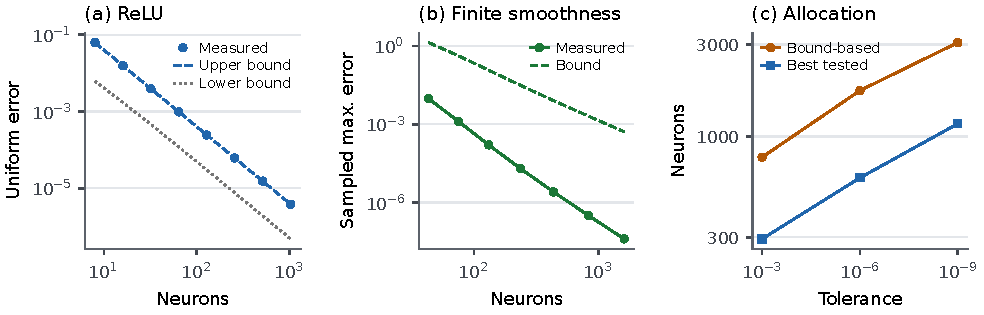
\includegraphics[width=0.97\linewidth]{../empirical/figures/additional_tests.pdf}
\small
\caption{\textbf{Other checks.} (a) ReLU's algebraic rate for $x^2$.
(b) A finite-smooth target with Gaussian kernels. (c) The sufficient allocation
versus the best measured configuration in the tested grid.}
\label{fig:other-tests}
\end{figure}

\textbf{Lambda consistency check.} A separate check uses the canonical
scalar profiles of \(e^{-3\|x\|^2}\) in \(d=1,2,3,4\), with 128 or 512
interval cells and \(R=n/4\). At 512 cells, \(\lambda=0.25\) gives relative
sampled profile errors between \(8.1\times10^{-16}\) and
\(5.3\times10^{-15}\); the halo-only balance \(2\pi/R\simeq0.0491\)
gives \(7.7\times10^{-13}\) to \(4.4\times10^{-11}\) in the same float64
implementation. This supports retaining the Fourier-ratio seed at working
precision. These are scalar-profile comparisons, not a full angular
reconstruction or a test of universal optimality. The check is reproduced by
\texttt{python empirical/lambda\_consistency.py}.

Reproduction requires Python, NumPy, SciPy, and Matplotlib. Run
\texttt{python empirical/run.py --suite all}, then
\texttt{python empirical/plot.py}. Configuration, all recorded results,
software versions, and a run log are included. The sphere weights and
polynomial moments are checked independently. Doubling contour quadrature
changed the analytic pilot predictions by at most \(1.3\times10^{-15}\);
this is a numerical diagnostic rather than an interval certificate.

\section{Proofs of the four main results}\label{sec:theorems}
The supporting lemmas are grouped by the result they establish.
Appendix~\ref{sec:source} derives the analytic profile bounds from the target
assumptions.

\subsection{Proof of analytic convergence: scalar and angular errors add}
\begin{lemma}[Positive-weight assembly and origin anchoring]\label{lem:assembly}
Suppose a target satisfies
\(f(x)=f(0)+\int H_x\dd\sigma\), with
\(H_x(\theta)=g_\theta(\theta\cdot x)-g_\theta(0)\).
Suppose \(\alpha_m\ge0\), \(\sum_m\alpha_m=1\), the angular error is uniformly
at most \(E_\theta\), and
\(\sup_{|s|\le1}|U_m(s)-g_{\theta_m}(s)|\le e_m\).
Then \eqref{eq:network} is exact at zero and
\begin{equation}\label{eq:assembly}
 \norm{\widehat f-f}_{L^\infty(\Ball)}
       \le E_\theta+2\sum_m\alpha_me_m.
\end{equation}
\end{lemma}
\begin{proof}
At zero every centered spoke is zero. At another point, insert and subtract
the quadrature sum of the exact centered profiles.
The angular difference is at most \(E_\theta\).
Each remaining centered spoke difference is bounded by \(e_m+e_m\).
Multiply by its nonnegative weight and sum. No factor equal to the number
of directions is introduced.
\end{proof}


\subsubsection{The scalar error and its finite halo}
\begin{lemma}[Frequency truncation, sampling, and halo errors]\label{thm:ledger}
Let \(K\) be a real Schwartz kernel, \(\gamma,h>0\), \(B\ge0\), and \(J\subset\Z\)
finite. Let \(\widehat p\in L^1(\R;\C)\), and assume
\(\widehat K(\xi/\gamma)\ne0\) for \(|\xi|\le B\). Define
\[
 b_B(\xi)=\mathbf1_{[-B,B]}(\xi)
             \frac{\widehat p(\xi)}{\widehat K(\xi/\gamma)},\qquad
 \rho=\mathcal F^{-1}b_B,\qquad K_\gamma(t)=\gamma K(\gamma t).
\]
Write \(p=\mathcal F^{-1}\widehat p\). Then at every real \(s\),
\begin{align}
 \left|p(s)-h\sum_{j\in J}\rho(jh)K_\gamma(s-jh)\right|
 \le{}&
 \underbrace{\int_{|\xi|>B}|\widehat p(\xi)|\dd\xi}_{E_{\rm cut}}\nonumber\\
 &+\underbrace{\sum_{k\in\Z\setminus\{0\}}\int_\R
       |b_B(\xi)|\,|\widehat K((\xi-k/h)/\gamma)|\dd\xi}_{E_{\rm alias}}\label{eq:ledger}\\
 &+\underbrace{h\norm{b_B}_{L^1}
       \sum_{j\notin J}|K_\gamma(s-jh)|}_{E_{\rm halo}}.\nonumber
\end{align}
The sums converge. Taking real parts gives the same bound for the real spoke sum.
If additionally (K1) holds, \(T>0\), \(g\in C^r([-T,T])\), and \(g^{(r)}=\operatorname{Re}p\)
there, the activation sum matching \(g\)'s derivatives of orders
\(0,\ldots,r-1\) at zero
has function error at most
\[
 \frac{T^r}{r!}\sup_{|s|\le T}
       (E_{\rm cut}+E_{\rm alias}+E_{\rm halo}).
\]
For \(r=0\) this is the kernel approximation itself and no anchor is needed.
\end{lemma}
\begin{proof}
Continuity and nonvanishing of the denominator on a compact interval give a
finite bound on its inverse, so \(b_B\in L^1\).
Its inverse transform is smooth with bounded derivatives, because every
frequency moment of \(b_B\) is integrable. For fixed \(s\), the product
\(\rho(c)K_\gamma(s-c)\) and its Fourier transform have sufficient decay for
Poisson summation. The scaled formula is
\[
 h\sum_{j\in\Z}\rho(jh)K_\gamma(s-jh)
 =\sum_{k\in\Z}\int_\R b_B(\xi)
       e^{2\pi\ii(\xi-k/h)s}\widehat K((\xi-k/h)/\gamma)\dd\xi.
\]
The \(k=0\) term is exactly
\(\int_{-B}^{B}\widehat p(\xi)e^{2\pi\ii\xi s}\dd\xi\): this is where
deconvolution cancels the kernel. Its difference from \(p(s)\) is bounded by
\(E_{\rm cut}\). Taking absolute values of the other terms gives \(E_{\rm alias}\).

Deleting indices outside \(J\) contributes at most \(E_{\rm halo}\), since
\(|\rho(c)|\le\norm{b_B}_1\). This proves \eqref{eq:ledger}.
The differentiated raw activation sum is exactly the retained kernel sum,
by \eqref{eq:derivative-kernel} and its coefficient prefactor.
Adding the anchor polynomial makes the error's derivatives of orders
\(0,\ldots,r-1\) vanish at zero. Taylor's integral remainder, or the
Lagrange remainder used in Lean, then bounds the error by
\(T^r/r!\) times the derivative error. The interior version of this argument
does not impose extra differentiability across the interval endpoints.
\end{proof}

For later constants, put
\[
 \mathcal T(b,\eta)=\int_0^\infty e^{-bt^\eta}\dd t
     =b^{-1/\eta}\Gamma(1+1/\eta),\qquad b,\eta>0,
\]
and define the fixed kernel constant
\begin{equation}\label{eq:Cker}
 C_{\rm ker}=1+\frac{C_K}{c_K}\bigl(1+2\mathcal T(2,\nu)\bigr)
       +\frac{2C_s}{c_K}\bigl(1+\mathcal T(b_K/2,\mu)\bigr).
\end{equation}

\begin{lemma}[Envelope suppression]\label{lem:envelope}
Use the kernel and integrable spectrum of Lemma~\ref{thm:ledger}.
Assume (K2)--(K3), \(T>0\), \(L\ge1\), \(B>0\),
\(\gamma=B/L^{1/\nu}\), \(h=1/(HB)\), \(D=ZL^{1/\mu}/\gamma\),
and the two inequalities following \eqref{eq:HZ}.
For the grid \(|j|\le\lfloor(T+D)/h\rfloor\), the alias and halo terms obey
\begin{align*}
 E_{\rm alias}
 &\le\norm{\widehat p}_1\frac{C_K}{c_K}
       (1+2\mathcal T(2,\nu))e^{-2L},\\
 \sup_{|s|\le T}E_{\rm halo}
 &\le\norm{\widehat p}_1\frac{2C_s}{c_K}
       (1+\mathcal T(b_K/2,\mu))e^{-3L}.
\end{align*}
If \(A_\sigma=\int e^{\sigma|\xi|}|\widehat p(\xi)|\dd\xi<\infty\),
\(\sigma>0\), and \(B=L/\sigma\), the anchored activation error is at most
\[
 A_\sigma C_{\rm ker}e^{-L}\frac{T^r}{r!}.
\]
Assume (K1) and the target/derivative agreement of Lemma~\ref{thm:ledger}
when applying the last assertion.
\end{lemma}
\begin{proof}
On the retained band, division by the kernel amplifies spectral mass by at
most \(c_K^{-1}e^{A_KL}\).
For \(k\ne0\) and \(|\xi|\le B\),
\[
 |\xi-k/h|\ge HB|k|-B\ge (H/2)B|k|.
\]
The ratio of the shifted kernel transform to the unshifted one is consequently
at most \((C_K/c_K)e^{-4L|k|^\nu}\).
Sum the positive and negative aliases and compare the decreasing tail with
its integral to obtain the first bound.

An omitted center has distance at least \(D\) from any \(s\in[-T,T]\), with
subsequent distances increasing in steps of \(h\). Since
\((u+v)^\mu\ge(u^\mu+v^\mu)/2\) for \(u,v\ge0\), the spatial exponential
separates into a halo suppression and a summable lattice tail.
The suppression is at most \(e^{-(A_K+3)L}\). After the inverse-kernel
factor \(e^{A_KL}\), it leaves \(e^{-3L}\).
The remaining lattice sum is bounded by its first term plus its integral;
\(\gamma h\le1\) gives the displayed constant and includes both halo sides.

Finally \(E_{\rm cut}\le A_\sigma e^{-\sigma B}=A_\sigma e^{-L}\) and
\(\norm{\widehat p}_1\le A_\sigma\). Adding the three terms and anchoring
proves the result.
\end{proof}

Let \(E_\delta=\{\cos z:|\operatorname{Im}z|\le\delta\}\), the closed filled
Bernstein ellipse. For \(T_0>1\), define
\begin{align}
 \omega_0&=T_0^{-2}-1-\log(T_0^{-2})>0,\nonumber\\
 b_{\rm sc}&=\min\{\delta/2,\omega_0/2,2\},\label{eq:scalar-rate}\\
 C_{\rm mom}(B_g,T_0,r)
   &=2B_g\sqrt{4\pi T_0^2}\,(2\pi)^r\,\frac{2r!}{\pi^{r+1}},\nonumber\\
 V(B_g,\delta,T_0,r)
   &=\frac{B_g(6+8/\delta)}{1-e^{-\delta}}
      +2B_g(1+2/\omega_0)
      +\frac{C_{\rm mom}(B_g,T_0,r)C_{\rm ker}}{r!}.\label{eq:V}
\end{align}
These constants are independent of \(n\).

\begin{lemma}[A finite spoke sum from local analytic samples]\label{thm:scalar}
Assume (K1)--(K3). Let \(g:\C\to\C\) be holomorphic on a neighborhood of
\(E_\delta\), with \(\delta>0\) and \(|g|\le B_g\) on that ellipse.
Use the real values \(\operatorname{Re}g(t_j)\) in the construction;
if \(g\) is real on the interval these are just its values.
Fix \(T_0>1\), \(n\ge1\), and \(H,Z\) satisfying the inequalities after
\eqref{eq:HZ}. Construct the finite spoke sum \(U_n\) by
\eqref{eq:prepared}--\eqref{eq:density} and the derivative anchor.
Then
\begin{equation}\label{eq:scalar-error}
 \sup_{|s|\le1}|U_n(s)-\operatorname{Re}g(s)|
 \le V(B_g,\delta,T_0,r)e^{-b_{\rm sc}n}.
\end{equation}
Put
\[
 \kappa_{\rm gen}=\max\{1,1/\mu+1/\nu\},\qquad
 C_{\rm grid}=(2H/\pi+2HZ+1)(G+3)^{\kappa_{\rm gen}}.
\]
The actual finite spoke sum, including both halos, has
\begin{equation}\label{eq:row-width}
 |J|\le C_{\rm grid}n^{\kappa_{\rm gen}}.
\end{equation}
This counts the grid neurons. A higher-order anchor's realization is a
separate requirement.
\end{lemma}
\begin{proof}
There are three steps.

First, composing \(g\) with the cosine turns its ellipse into a periodic
strip. Shift the Fourier coefficient integral to the upper or lower boundary
of that strip. The Chebyshev coefficients are bounded by \(2B_ge^{-\delta k}\).
Truncating their series after degree \(n\) has error at most
\(2B_ge^{-\delta(n+1)}/(1-e^{-\delta})\).
Discrete Chebyshev orthogonality proves that the sample polynomial reproduces
every polynomial of degree at most \(n\). Its operator norm on bounded samples
is at most \(2(n+1)\). Applying reproduction to the truncated series gives
\[
 \norm{P_n-\operatorname{Re}g}_\infty
 \le\frac{B_g(4n+6)e^{-\delta n}}{1-e^{-\delta}}
 \le\frac{B_g(6+8/\delta)}{1-e^{-\delta}}e^{-\delta n/2}.
\]
For complex \(g\), the same argument applies to its real restriction by
taking real parts of the approximating polynomial; the reproduction and
norm estimates are real.

Second, for \(0\le u\le T_0^{-2}<1\), the truncated exponential satisfies
\[
 0\le e^{-nu}\sum_{k=0}^{n}\frac{(nu)^k}{k!}\le1,\qquad
 1-e^{-nu}\sum_{k=0}^{n}\frac{(nu)^k}{k!}
 \le e^{-n(T_0^{-2}-1-\log T_0^{-2})}.
\]
To see the tail bound, compare its \(k\ge n+1\) terms with
\(u^n n^k/k!\), sum, and multiply by \(e^{-nu}\).
Since \(|P_n|\le2B_g(n+1)\), the window changes the polynomial on the interval
by at most
\[
 2B_g(n+1)e^{-\omega_0n}
 \le2B_g(1+2/\omega_0)e^{-\omega_0n/2}.
\]

Third, one must account for the size of the prepared spectrum.
Bounding the Chebyshev polynomials by \((1+2|z|)^k\), and absorbing their real
growth into half of the Gaussian decay, gives, on \(z=x\pm\ii\),
\[
 |u_n(z)|\le2B_g(n+1)e^{Gn}
                      e^{-nx^2/(4T_0^2)}.
\]
Horizontal contour shifting therefore gives
\[
 |\widehat u_n(\xi)|
 \le2B_g(n+1)e^{Gn}\sqrt{4\pi T_0^2/n}\,e^{-2\pi|\xi|}.
\]
The vertical sides vanish by the displayed Gaussian bound.
Multiplication by the derivative factor \((2\pi|\xi|)^r\), followed by
integration against \(e^{\pi|\xi|}\), proves
\[
 \int_\R e^{\pi|\xi|}|\widehat p_n(\xi)|\dd\xi
 \le C_{\rm mom}(B_g,T_0,r)e^{(G+1)n}.
\]
Here \(n+1\le e^n\), \(n^{-1/2}\le1\), and
\(\int_\R|\xi|^re^{-\pi|\xi|}\dd\xi=2r!/\pi^{r+1}\).
Thus the accuracy-dependent spectral norm is explicitly controlled.
Lemma~\ref{lem:envelope}, with \(L=(G+3)n\), makes the prepared-function
approximation error at most
\(C_{\rm mom}C_{\rm ker}e^{-2n}/r!\).
Adding the interpolation, window, and kernel errors yields \eqref{eq:scalar-error}.

Finally,
\[
 |J|=2\lfloor(1+D)/h\rfloor+1
 \le \frac{2H}{\pi}L+2HZL^{1/\mu+1/\nu}+1
 \le(2H/\pi+2HZ+1)L^{\kappa_{\rm gen}}.
\]
Substitute \(L=(G+3)n\) to obtain \eqref{eq:row-width}.
\end{proof}

\subsubsection{The corrected tanh scalar construction}\label{sec:corrected-tanh}
We derive the finite-halo correction used in the experiments and its error
bound. This is the part of the tanh result not yet formalized in Lean.

\paragraph{Coefficients.}
Assume a scalar profile \(g\) is holomorphic and bounded by \(B\) on the
complex \(\delta\)-neighborhood of \([-1-\Delta,1+\Delta]\), is real on
that real interval, and can be evaluated there, with \(\delta,\Delta>0\).
The coefficient formulas and three-term error bound below apply for any
\(h=2/n\), \(\gamma>0\), and integer halo count \(R\) satisfying
\eqref{eq:lambda-admissible}, with \(\lambda=\gamma h\).
The following particular schedule balances the two exponential factors
and is used to derive the width law.
Fix \(0<\ell_0\le\min(\delta/2,\Delta/2)\), a physical halo length, and set
\[
 \gamma=2\pi/\ell_0,\quad \tau=\pi/(2\gamma)=\ell_0/4,\quad
 h=2/n,\quad\lambda=\gamma h=4\pi/(\ell_0 n),\quad
 R=\lceil \ell_0 n/2\rceil,\quad c_j=-1+jh.
\]
Take \(n\ge\lceil\max(16,4\pi/\ell_0,3/(\Delta-\ell_0))\rceil\).
Then \(\lambda\le1\), \(\gamma\delta\ge4\pi\), and the actual halo extent
\(\ell_h=(R+1/2)h\) is at most \(\Delta\).
There are exactly \(N=n+1+2R\le(1+\ell_0)n+3\) neurons.
Write \(a=-1-\ell_h\), \(b=1+\ell_h\), and initialize
\[
 \rho(z)=\frac{g(z+\ii\tau)-g(z-\ii\tau)}{2\ii\tau},
 \qquad u_j=\frac h2\rho(c_j),\qquad -R\le j\le n+R.
\]
The density is real at real centers. It is an exact deconvolution identity
for this activation, not a small-step finite-difference approximation.

Set \(k_0=\lceil\delta/(8\tau)\rceil\), \(\sigma=2k_0\tau\), and
\(L=\lfloor(R+1)/2\rfloor\). For \((e,\epsilon)=(a,+1),(b,-1)\), compute
\begin{align*}
 \mu_\ell(e,\epsilon)&=\frac1{2\tau}\int_{-\tau}^{\tau}
       g(e+\ii y)e^{2\ii\epsilon\ell\gamma y}\dd y,\\
 \nu_\ell(e,\epsilon)&=2(-1)^\ell\operatorname{Im}\int_0^\sigma
       \frac{\rho(e+\ii y)e^{2\ii\epsilon\ell\gamma y}}
       {1+e^{2\pi y/h}}\dd y,\qquad 1\le\ell\le L,\\
 G_\ell^-&=\mu_\ell(a,+1)-\nu_\ell(a,+1),\qquad
 G_\ell^+=\mu_\ell(b,-1)-\nu_\ell(b,-1).
\end{align*}
Subtracting the constant \(g(e)\) in the \(\mu\) integral changes nothing and
improves its numerical evaluation. All these integrals are one-dimensional
and over finite segments inside the assumed complex neighborhood.

Put \(z_0=e^{-2\lambda}\), \(r_i=z_0^{i-1/2}\), and
\(p_j=\prod_{k=1}^j(1-z_0^k)\), with \(p_0=1\).
Let \(e_j(r_{-i})\) denote the coefficient of \(z^j\) in
\(\prod_{k\ne i}(1+r_kz)\). Finite polynomial multiplication gives these
numbers. Compute
\[
 \kappa_i^\pm=
 \frac{(-1)^i z_0^{[i(i+1)-1]/2}}{p_{i-1}p_{L-i}}
       \sum_{\ell=1}^L G_\ell^\pm e_{\ell-1}(r_{-i}),\qquad 1\le i\le L.
\]
Modify only the outer halo slots:
\[
 u_{-R+i-1}\mathrel{+}=\kappa_i^-/2,\qquad
 u_{n+R-i+1}\mathrel{-}=\kappa_i^+/2.
\]
Finally set \(b_g=g(-1)-\sum_j u_j\tanh(\gamma(-1-c_j))\).
The result is the ordinary network
\(Q_g(s)=b_g+\sum_j u_j\tanh(\gamma(s-c_j))\).
No polynomial or rational function is evaluated outside this network.

\paragraph{Why the correction works.}
For \(s_0=-1\), define
\[
 D_s(z)=\tfrac12[\tanh(\gamma(s-z))-\tanh(\gamma(s_0-z))],\qquad
 H_s(z)=\coth(\gamma(s-z))-\coth(\gamma(s_0-z)).
\]
The identity \(H_s(t\pm\ii\tau)=2D_s(t)\), followed by the residue theorem
on \([a,b]+\ii[-\tau,\tau]\), gives
\[
 g(s)-g(s_0)=\int_a^b\rho(t)D_s(t)\dd t+\mathcal B(s),
\]
\[
 \mathcal B(s)=\frac1{4\tau}\int_{-\tau}^{\tau}
 [g(a+\ii y)H_s(a+\ii y)-g(b+\ii y)H_s(b+\ii y)]\dd y.
\]
The residues of \(g(z)H_s(z)\) at \(s,s_0\) are
\(-g(s)/\gamma,g(s_0)/\gamma\); these and \(4\gamma\tau=2\pi\)
fix the factors and signs.

Midpoint quadrature has an endpoint contribution too. To see it, integrate
\(F_s(z)=\rho(z)D_s(z)\) against
\[
 \mathcal K_h(z)=\frac1{2\ii}\cot\frac{\pi(z-a-h/2)}h,
 \qquad R_h^\pm=\mathcal K_h\pm\tfrac12
\]
on the rectangle of height \(\sigma\). The grid poles have residues
\(h/(2\pi\ii)\), so they produce the midpoint sum. Separating the upper
and lower halves gives the exact signed identity
\[
 h\sum_jF_s(c_j)-\int_a^bF_s(t)\dd t
       =\mathcal H_h+\mathcal V_h-\mathcal P_h.
\]
Here \(\mathcal H_h\) comprises the two horizontal contour integrals,
\(\mathcal P_h\) is \(2\pi\ii\) times the enclosed non-grid residues of
\(R_h^+F_s\) above and \(R_h^-F_s\) below, and
\[
 \mathcal V_h=\ii\int_0^\sigma
 \frac{F_s(b+\ii y)-F_s(a+\ii y)-F_s(b-\ii y)+F_s(a-\ii y)}
      {1+e^{2\pi y/h}}\dd y.
\]
Thus the boundary term to cancel is \(\mathcal B-\mathcal V_h\).
Expanding coth and tanh at the endpoints writes it as the four anchored
values of the two series \(G^\pm(z)=\sum_{\ell\ge1}G_\ell^\pm z^\ell\),
at \(z_-(s)=e^{-2\gamma(s-a)}\) and
\(z_+(s)=e^{-2\gamma(b-s)}\). The coth series gives \(\mu\), the tanh
series in \(\mathcal V_h\) gives \(\nu\), and their difference gives exactly
the moments above. Uniform convergence at these endpoints justifies the
termwise integrals.

Let \(t_i=1/r_i\), \(D_L(z)=\prod_i(1+t_i z)\), and
\(P_L^\pm=[D_LG^\pm]_{\le L}\). The prescribed rational functions
\(P_L^\pm/D_L\) match the first \(L\) boundary coefficients. Their partial
fractions are a constant plus \(\sum_i\kappa_i^\pm/(1+t_i z)\).
Multiplication by \(1+t_i z\) and evaluation at \(-1/t_i\) gives the
coefficient formula; expressing the other factors using \(r_i\) gives
its scaled form above. Finally,
\[
 \frac1{1+t_i z_-(s)}=\frac{1+\tanh(\gamma(s-c_{-R+i-1}))}{2},
 \qquad
 \frac1{1+t_i z_+(s)}=\frac{1-\tanh(\gamma(s-c_{n+R-i+1}))}{2}.
\]
The constant parts cancel under anchoring. This proves that the rational
correction is precisely the stated change to ordinary tanh readouts.

\paragraph{Error and width.}
Cauchy's derivative bound gives \(|\rho|\le4B/\delta\) on the contour.
The contour factors satisfy
\(|R_h^\pm(z)|\le(e^{2\pi|\operatorname{Im}z|/h}-1)^{-1}\)
in their respective half-planes. Since \(\gamma\sigma=k_0\pi\), the
horizontal values of \(D_s\) equal their real values, whose integral is at
most two. The non-grid poles lie at heights \((2j+1)\tau\), with residue
moduli \(1/(2\gamma)\). These observations give
\[
 E_{\rm hor}\le\frac{32B}{\delta}e^{-\pi\delta n/4},\qquad
 E_{\rm pole}\le\frac{64\pi B}{\lambda\delta n}e^{-\pi^2/\lambda}.
\]
For the pole bound, sum
\(\sum_{j\ge0}(e^{(2j+1)\pi^2/\lambda}-1)^{-1}
\le2e^{-\pi^2/\lambda}\), valid for \(\lambda\le1\).

For the correction error, subtract \(g(e)\) in \(\mu_\ell\) and use
Cauchy's derivative estimate, then integrate the logistic factor in \(\nu\):
\[
 |G_\ell^\pm|\le M_h:=\frac{Bh}{\delta}D_\lambda,
 \qquad D_\lambda=\frac\pi{2\lambda}+\frac{4\log2}{\pi}.
\]
Put \(\vartheta=e^{-\gamma\ell_h}\). On \(|z|=\vartheta\),
\(|D_L(z)|\le2^L\) and \(|G^\pm(z)|\le M_h/(1-\vartheta)\).
Cauchy's coefficient estimate for the terms beyond degree \(L\), evaluated
at \(0\le z\le\vartheta^2\), gives
\[
 |G^\pm(z)-P_L^\pm(z)/D_L(z)|
 \le\frac{M_h\vartheta}{(1-\vartheta)^2}(2\vartheta)^L.
\]
We used \(D_L(z)\ge1\) on this real interval. There are four anchored
endpoint evaluations. Since \(\lambda R\ge2\log2\) and \(L\ge R/2\),
the resulting error is at most
\[
 E_{\rm halo}\le16M_h e^{-\lambda R^2/4}
          =\frac{32BD_\lambda}{\delta n}e^{-\lambda R^2/4}.
\]
Their sum bounds \(\|g-Q_g\|_\infty\).

Set \(\beta=\pi \ell_0/4\). Under the displayed schedule,
\[
 \pi\delta n/4\ge2\beta n,\qquad
 \pi^2/\lambda=\beta n,\qquad
 \lambda R^2/4\ge\beta n.
\]
The remaining factors are uniformly bounded in \(n\), yielding
\[
 \|g-Q_g\|_\infty\le(32/\delta+12)B e^{-\beta n},\qquad
 N\le(1+\ell_0)n+3.
\]
Positive angular assembly now gives
\(E\le Ue^{-aq}+2(32/\delta+12)B e^{-\beta n}\) and
\(W\le q^{d-1}[(1+\ell_0)n+3]\). Choosing both orders proportional to
\(\log(1/\eps)\) proves the \(d\) exponent. The scalar hypothesis must hold
uniformly over the selected profiles, with fixed constants and margins.
It follows from a common complex neighborhood of those profiles; shrinking
it with the tolerance would change this conclusion.

This improvement uses \(R\asymp n\) and \(\lambda\asymp1/n\), not a fixed
\(\lambda\) with square-root halos. The physical halo remains bounded.
It does not guarantee numerical stability at fixed precision: the moment-to-readout
map has a bound growing like
\(\sqrt{\ell_0 n}\exp(5\pi \ell_0 n/96)\). More working bits may be required as the
requested accuracy increases. The companion
\path{docs/sharper_tanh.md} records this conditioning calculation and absolute
coefficient-error budgets in detail.

\begin{lemma}[Corrected tanh after finite sample preparation]\label{lem:tanh-prepared}
Use the analytic preparation \(u_n\) in \eqref{eq:prepared}, with the
hypotheses of Lemma~\ref{thm:scalar}. Set \(\beta_0=\pi/8\),
\[
 m_n=\left\lceil\max\{32,(G+3)n/\beta_0\}\right\rceil,\qquad
 C_{\tanh}=\tfrac32\max\{32,(G+3)/\beta_0\}+\tfrac92.
\]
Apply the corrected tanh construction to \(u_n\), with interval-cell count
\(m_n\), strip bound \(\delta=1\), real margin \(\Delta=1\), and physical
halo \(\ell_0=1/2\). The result has at most \(C_{\tanh}n\) neurons and error
at most \(V_{\tanh}e^{-b_{\rm sc}n}\) from \(\operatorname{Re}g\) on the real interval, where
\[
 V_{\tanh}=
 \frac{B_g(6+8/\delta_g)}{1-e^{-\delta_g}}
 +2B_g(1+2/\omega_0)+88B_g.
\]
Here \(\delta_g\) is the original profile's ellipse parameter; the strip
parameter for the entire prepared function is one.
For the finite-smooth preparation in Lemma~\ref{thm:algebraic-row}, the same
construction at preparation order \(2n\) has at most \(2C_{\tanh}n\)
neurons and error at most \(V_{\rm alg}^{\tanh}n^{-s_0}\), with
\[
 V_{\rm alg}^{\tanh}=4A_p+3B_gE(2\omega_0,s_0)+264B_gE(4,s_0).
\]
\end{lemma}
\begin{proof}
The preparation proof bounds the entire function on the full strip
\(|\operatorname{Im}z|\le1\), not merely at real points:
\[
 |u_n(z)|\le2B_g(n+1)e^{Gn}
               e^{-n(\operatorname{Re}z)^2/(4T_0^2)}
 \le2B_g e^{(G+1)n}.
\]
This follows directly from the Chebyshev growth and complex window estimates
used above; they are uniform for \(|\operatorname{Im}z|\le1\).
Thus the preceding corrected scalar bound applies with
\(B=2B_g e^{(G+1)n}\), despite that bound growing with preparation order.
The chosen number of cells compensates for this growth:
\[
 \|Q_{u_n}-u_n\|_\infty
 \le44\,[2B_g e^{(G+1)n}]\,e^{-\beta_0m_n}
 \le88B_ge^{-2n}.
\]
Add the interpolation and window errors already proved in
Lemma~\ref{thm:scalar}. Since \(b_{\rm sc}\le2\), their sum is bounded
by \(V_{\tanh}e^{-b_{\rm sc}n}\).
The count follows from \(N\le\tfrac32m_n+3\), the ceiling inequality,
and \(n\ge1\).

For finite-smooth data, the filtered sample polynomial has real supremum
at most \(3B_g\) and is prepared at order \(2n\). Its strip bound is
\(6B_g e^{2(G+1)n}\), so the corrected-network error is at most
\(264B_g e^{-4n}\). Add its approximation and window errors
\(4A_pn^{-s_0}+3B_ge^{-2\omega_0n}\), then use
\(e^{-bn}\le E(b,s_0)n^{-s_0}\). This proves the stated algebraic constant
and linear count. The construction uses the original finite real samples;
complex evaluations concern only their explicit entire preparation.
\end{proof}
Thus the correction gives a linear scalar count for both analytic and
finite-smooth preparation.

\subsubsection{The direction rule and its error}
\begin{lemma}[Positive spherical quadrature]\label{thm:directions}
For every \(d\ge2\) and integer \(q\ge1\), the rule in Section~\ref{sec:construction} has positive
weights summing to one. Its full \(2q^{d-1}\)-node version integrates every
spherical polynomial of degree at most \(2q-1\) exactly.
For any even integrand, folding preserves the weighted sum and leaves
\(q^{d-1}\) direction indices.
\end{lemma}
\begin{proof}
The positive interval weight defines a positive-definite inner product on
polynomials, so Gram--Schmidt produces a monic orthogonal polynomial of each
degree. The degree-\(q\) orthogonal polynomial has
\(q\) distinct roots in the open interval. Otherwise, multiplying together
its sign-changing factors would produce a polynomial of lower degree whose
product with it has one sign and nonzero integral, contradicting orthogonality.

Temporarily define the node weights by \(\lambda_j=\int L_j\).
Divide a polynomial \(p\) of degree at most \(2q-1\) by this orthogonal
polynomial: \(p=av+r\), with \(\deg a,\deg r<q\).
The \(av\) integral vanishes and its values at all nodes vanish. Interpolate
\(r\) in the cardinal polynomials \(L_j\), which proves exactness.
Applying exactness to \(L_j^2\) identifies these weights with the
\(\int L_j^2\) formula used by the construction, and makes them strictly
positive; applying it to one gives normalization.

On the circle, summing \(e^{\ii k2\pi j/(2q)}\) over the \(2q\) nodes gives
zero for \(0<|k|<2q\). This proves the base case.
For the higher-dimensional recursion, check a coordinate monomial.
If its total degree in the lower-sphere coordinates is odd, the lower-sphere
integral and discrete sum both vanish. If it is even, say \(2j\), the factor
from those coordinates is \((1-t^2)^j\). The remaining integrand in \(t\)
is a polynomial of degree at most \(2q-1\), so Gauss--Jacobi is exact.
Induction proves full spherical exactness and the product node count.
Antipodal equality permits adding paired weights for even functions.
\end{proof}

Let \(H_\ell\) denote the canonical degree-\(\ell\) spherical harmonic
component of a continuous function \(H:\Sph\to\R\), in \(L^2(\sigma)\).
These components are the orthogonal projections of \(H\); they are not supplied
as freely chosen coefficients. Restricted polynomials contain the constants
and separate points of the sphere, so Stone--Weierstrass gives density in
continuous functions and hence in \(L^2\). Splitting those polynomials into
orthogonal harmonic layers gives the complete canonical expansion.
The addition theorem gives
\begin{equation}\label{eq:addition}
 \norm{H_\ell}_\infty\le\sqrt{D_{d,\ell}}\norm{H_\ell}_2,\qquad
 \sum_{\ell\ge0}D_{d,\ell}z^\ell=\frac{1+z}{(1-z)^{d-1}},\quad 0\le z<1.
\end{equation}
One way to obtain the first identity is to sum squares of an orthonormal
basis of a harmonic layer. Rotations preserve the sum and act transitively
on the sphere, so it is constant; integration identifies that constant with
the dimension. Orthogonal complements of successive polynomial spaces give
the dimensions:
\[
 D_{d,\ell}=\binom{d+\ell-1}{\ell}-\binom{d+\ell-3}{\ell-2},
\]
with the second term zero for \(\ell<2\). Their generating function is
\((1-z^2)/(1-z)^d=(1+z)/(1-z)^{d-1}\).

\begin{lemma}[Angular quadrature error]\label{thm:angular}
Let \(H:\Sph\to\R\) be continuous and even, \(q\ge1\), and \(Q_q\) the
folded rule. In the analytic case assume, for \(a>0\), \(A_\theta\ge0\),
\[
 \sum_{\ell\ge0}e^{2a\ell}\norm{H_\ell}_2^2\le A_\theta^2.
\]
Then
\begin{equation}\label{eq:analytic-angular}
 \left|\int H\dd\sigma-Q_qH\right|
 \le A_\theta
 \sqrt{\frac{1+e^{-a}}{(1-e^{-a})^{d-1}}}\,e^{-aq}.
\end{equation}
In the Sobolev case assume \(A_\theta\ge0\), \(s_\theta>(d-1)/2\), and
\[
 \sum_{\ell\ge0}(1+\ell)^{2s_\theta}\norm{H_\ell}_2^2\le A_\theta^2.
\]
Set \(t=s_\theta-(d-1)/2>0\) and
\(C_d=\sqrt{2(d-1)^{d-2}}\). Then
\begin{equation}\label{eq:sobolev-angular}
 \left|\int H\dd\sigma-Q_qH\right|
 \le\frac{C_dA_\theta}{\sqrt{2t}}(2q-1)^{-t}
 \le\frac{C_dA_\theta}{\sqrt{2t}}q^{-t}.
\end{equation}
\end{lemma}
\begin{proof}
The weighted assumptions and \eqref{eq:addition} make the harmonic series
uniformly absolutely convergent. Its continuous sum equals \(H\):
the canonical orthogonal expansion already equals \(H\) in \(L^2\), and
a continuous difference with zero \(L^2\) norm is zero everywhere, because
surface measure assigns positive mass to every nonempty open set.
This prevents a merely almost-everywhere statement from being used at nodes.

Let \(P=\sum_{\ell<2q}H_\ell\). Its constant component contains the complete
spherical mean; all positive-degree harmonics have zero integral.
Thus \(\int P=\int H\), and Lemma~\ref{thm:directions} gives
\[
 \int H-Q_qH=Q_q(P-H),\qquad
 |\int H-Q_qH|\le\norm{P-H}_\infty.
\]
Positive normalized weights are essential to the last step.

In the analytic case, Cauchy--Schwarz gives
\[
 \norm{H-P}_\infty
 \le A_\theta\left(\sum_{\ell\ge2q}D_{d,\ell}e^{-2a\ell}\right)^{1/2}.
\]
For \(\ell\ge2q\), \(e^{-2a\ell}\le e^{-2aq}e^{-a\ell}\).
Insert the generating function in \eqref{eq:addition} to get
\eqref{eq:analytic-angular}. The sharper tail series is also a valid
intermediate bound.

For the Sobolev case, the binomial dimension formula yields
\(D_{d,\ell}\le C_d^2(1+\ell)^{d-2}\).
Cauchy--Schwarz and the integral comparison for the decreasing tail give
\[
 \norm{H-P}_\infty
 \le C_dA_\theta
 \left(\sum_{\ell\ge2q}(1+\ell)^{d-2-2s_\theta}\right)^{1/2}
 \le\frac{C_dA_\theta}{\sqrt{2t}}(2q-1)^{-t}.
\]
Using \(2q-1\) as the lower integration endpoint gives the stated bound.
Since \(2q-1\ge q\), the simpler power bound follows.
\end{proof}

\subsubsection{Combine the bounds and count all neurons}
\begin{proof}[Proof of Theorem~\ref{thm:main}]
Lemma~\ref{thm:source} supplies the scalar and angular hypotheses for the
target, uniformly over the unit ball.
Apply Lemma~\ref{thm:scalar} for the general recipe or
Lemma~\ref{lem:tanh-prepared} for corrected tanh to every retained direction, then
Lemma~\ref{thm:angular} and Lemma~\ref{lem:assembly}.
The scalar errors are all bounded by \(Ve^{-bn}\), so their weighted sum
is bounded by the same number. The cardinality is the product of the
\(q^{d-1}\) direction indices and the full scalar grid count.
This proves \eqref{eq:main-finite}.

For a requested \(\eps>0\), define, with \(\log0=0\) solely in this order rule,
\[
 \ord(C,b,\eta)
   =\left\lceil\max\left\{1,\frac{\max\{1,\log(C/\eta)\}}{b}\right\}\right\rceil,
\]
and choose
\begin{equation}\label{eq:orders}
 q=\ord(U,a,\eps/2),\qquad n=\ord(V,b,\eps/4).
\end{equation}

For \(C\ge0\), \(b,\eta>0\), the selected order satisfies
\(Ce^{-b\ord(C,b,\eta)}\le\eta\). If \(C=0\) this is immediate; otherwise
the order is at least \(\log(C/\eta)/b\).
The two budgets in \eqref{eq:orders} consequently give
\(\eps/2+2(\eps/4)=\eps\).

To make the count quantitative, for \(0<\eps\le e^{-1}\) set
\[
 D(C,b)=(1+1/b)\bigl(1+|\log\max\{1,2C\}|\bigr).
\]
The elementary ceiling bound proves
\[
 \ord(C,b,\eps/2)\le D(C,b)|\log\eps|.
\]
The coefficient \(1+1/b\) follows by considering whether
\(\max(1,\log(C/(\eps/2)))/b\) is below one, then using
\(\lceil z\rceil\le z+1\).
Also \(\ord(V,b,\eps/4)=\ord(2V,b,\eps/2)\).
Thus the actual grid after upward rounding satisfies
\begin{equation}\label{eq:explicit-width}
 W_{\rm grid}\le CD(U,a)^{d-1}D(2V,b)^\kappa
                       |\log\eps|^{d-1+\kappa}.
\end{equation}
All constants are fixed before \(\eps\) varies, proving \eqref{eq:geometric-width}.
The ordinary-MLP claim for \(r\le1\) follows directly by flattening the
direction and center indices in the final assembly in Section~\ref{sec:construction}.
\end{proof}

\begin{corollary}[Ordinary GELU network from a known target]\label{cor:gelu}
Under precisely the target hypotheses of Lemma~\ref{thm:source},
the prescribed construction with standard GELU, \(T_0=2\), and
\eqref{eq:HZ} yields, for every \(\eps>0\), one ordinary shallow MLP satisfying
\[
 \widehat f(0)=f(0),\qquad
 \norm{\widehat f-f}_{L^\infty(\Ball)}\le\eps,\qquad
 W\le W_{\rm grid}+2=O(\log^d(1/\eps)).
\]
The target assumptions determine all profile bounds and construction parameters.
\end{corollary}
\begin{proof}
Write \(\varphi(s)=(2\pi)^{-1/2}e^{-s^2/2}\) and
\(\Phi(s)=\int_{-\infty}^s\varphi(t)\dd t\).
For \(\GELU(s)=s\Phi(s)\),
\[
 \GELU''(s)=(2-s^2)\varphi(s),\qquad
 \widehat K(\xi)=(1+4\pi^2\xi^2)e^{-2\pi^2\xi^2}.
\]
The transform identity follows by writing \(K=\varphi-\varphi^{\prime\prime}\).
Thus \(r=2,\zeta=1\), with \(\nu=\mu=2\).
Verified choices are
\[
 c_K=1,\ C_K=5,\ A_K=2\pi^2,\ a_K=\pi^2,\quad
 C_s=6/\sqrt{2\pi},\ b_K=1/4 .
\]
Hence \(\kappa=1\). The target margins in
\eqref{eq:source-choice} and kernel choices \eqref{eq:HZ} satisfy all
construction parameter conditions.

The combined degree-one anchor is affine in \(x\).
Because \(\Phi(-s)=1-\Phi(s)\), GELU satisfies
\(\GELU(s)-\GELU(-s)=s\).
Two hidden neurons with opposite incoming vectors represent its linear part;
the constant joins the output bias. Apply \eqref{eq:explicit-width}.
\end{proof}

\begin{lemma}[Representing the integration polynomial]\label{thm:anchor}
Assume the hypotheses of Theorem~\ref{thm:main} for an arbitrary \(r\).
Let \(P_\eps(x)\) be the combined, centered degree-below-\(r\) integration
polynomial of the prescribed finite construction.
Suppose an ordinary network with the same activation and \(K_\eps\) additional
hidden neurons approximates this particular polynomial uniformly on \(\Ball\)
with error at most \(\eta\).
Replacing \(P_\eps\) by that network produces an ordinary one-hidden-layer MLP
with at most \(W_{\rm grid}+K_\eps\) neurons and total error at most the
grid-construction error plus \(\eta\).
\end{lemma}
\begin{proof}
The difference between the two evaluators is exactly the anchor-approximation
error. Add this to the already proved grid error by the triangle inequality.
The sum is one shallow network containing both sets of hidden neurons.
\end{proof}
The anchor's error and neuron count must be included for the chosen activation.
GELU represents it exactly with two neurons.

\begin{corollary}[Gaussian, cumulative Gaussian, and tanh]\label{cor:activations}
Under the analytic target assumptions of Lemma~\ref{thm:source}:
\begin{enumerate}
\item The raw Gaussian \(\phi(s)=e^{-\pi s^2}\), with \(r=0\), and Gaussian
      integral activations with \(r=1\), have \(\nu=\mu=2\). They give ordinary
      networks with \(W=O(\log^d(1/\eps))\).
\item Corrected tanh gives an ordinary network with exact origin anchoring
      and width \(O(\log^d(1/\eps))\).
\end{enumerate}
\end{corollary}
\begin{proof}
Differentiation under the Gaussian Fourier integral and integration by parts
give \(I^{\prime}(\xi)=-2\pi\xi I(\xi)\), with \(I(0)=1\) from the Gaussian integral. Hence
\(\mathcal F(e^{-\pi s^2})(\xi)=e^{-\pi\xi^2}\).
The standard normal density is its rescaling; it is the derivative of
the normal CDF. These kernels satisfy (K2)--(K3) with exponents two.
Their anchor order is at most one, so Theorem~\ref{thm:main} applies
without additional hidden units.

For tanh,
\[
 \phi'=2K,\qquad K(s)=\tfrac12\operatorname{sech}^2s,\qquad
 \widehat K(\xi)=
 \begin{cases}\pi^2\xi/\sinh(\pi^2\xi),&\xi\ne0,\\1,&\xi=0.\end{cases}
\]
For the transform, set \(u=e^{2s}\). Then \(K(s)\dd s=\dd u/(1+u)^2\), so
\[
 \widehat K(\xi)=\int_0^\infty\frac{u^{-\pi\ii\xi}}{(1+u)^2}\dd u
   =\Gamma(1-\pi\ii\xi)\Gamma(1+\pi\ii\xi).
\]
The beta integral and gamma reflection identity give the displayed hyperbolic
formula; the value at zero follows by continuity. The real bounds
\[
 e^{-\pi^2|\xi|}\le\widehat K(\xi)
       \le4e^{-(\pi^2/2)|\xi|},\qquad
 |K(s)|\le2e^{-2|s|}
\]
follow from the exponential formula for \(\sinh\).
Hence the generic estimate has \(\kappa_{\rm gen}=2\). Applying the
finite-halo correction and Lemma~\ref{lem:tanh-prepared} instead gives
\(\kappa=1\); no polynomial anchor neurons are needed because \(r=1\).
\end{proof}

\subsection{Proof of algebraic convergence and activation limits}
The following assumption is a specified approximation class, not a claim
about every nonanalytic function:
\begin{equation}\label{eq:poly-class}
 |g(s)|\le B_g\ (|s|\le1),\qquad
 \inf_{\deg P<n}\norm{g-P}_{L^\infty[-1,1]}\le A_p n^{-s_0}
 \quad(n\ge1),
\end{equation}
where \(A_p,B_g\ge0\) and \(s_0>0\). The Lean statement assumes that for each
\(n\) there exists a polynomial attaining the stated bound. Such polynomials,
or a slightly enlarged \(A_p\), connect the infimum formulation to that statement.

\begin{lemma}[Stable real-sample scalar construction]\label{thm:algebraic-row}
Assume (K1)--(K3), \eqref{eq:poly-class} with the approximating polynomials just specified,
\(T_0>1\), and the same \(H,Z\) inequalities.
There is an explicit spoke sum determined by \(2n\) real values of \(g\) such that
\[
 \norm{U_n-g}_\infty\le V_{\rm alg} n^{-s_0},\qquad
 |J|\le C_{\rm grid}(2n)^{\kappa_{\rm gen}},
\]
where
\begin{align*}
 E(b,s)&=\frac{\lceil s\rceil!}{b^{\lceil s\rceil}},\\
 V_{\rm alg}
 &=4A_p+3B_g E(2\omega_0,s_0)
       +\frac{C_{\rm mom}(3B_g,T_0,r)C_{\rm ker}}{r!}E(4,s_0).
\end{align*}
No complex evaluation of \(g\) is required.
\end{lemma}
\begin{proof}
Let \(\mathcal F_{m,L}\) be the sampled Fej\'er operator in the Chebyshev
coordinate, using \(L\) Chebyshev roots. Its kernel is positive and has
sampled mass one. Hence its operator norm on \([-1,1]\) is at most one.
The finite filter
\[
 \mathcal V_ng=2\mathcal F_{2n,2n}g-\mathcal F_{n,2n}g
\]
has norm at most three. For a Chebyshev mode of degree \(k<n\), its multiplier
is \(2(1-k/(2n))-(1-k/n)=1\), by discrete orthogonality.
It therefore reproduces every polynomial of degree below \(n\).
For an approximating polynomial \(P\) in \eqref{eq:poly-class},
\[
 \norm{g-\mathcal V_ng}_\infty
 =\norm{(g-P)-\mathcal V_n(g-P)}_\infty\le4A_pn^{-s_0}.
\]
Also \(\norm{\mathcal V_ng}_\infty\le3B_g\) and its degree is at most \(2n\).

Apply the preceding polynomial/window construction with preparation order
\(2n\) to this already computed polynomial. Re-interpolation reproduces it
exactly; it does not request new values of the original \(g\).
The window and kernel estimates from the previous proof give
\[
 \norm{U_n-g}_\infty
 \le4A_pn^{-s_0}+3B_ge^{-2\omega_0n}
       +\frac{C_{\rm mom}(3B_g,T_0,r)C_{\rm ker}}{r!}e^{-4n}.
\]
For \(x\ge1\), \(b>0\), and \(k=\lceil s_0\rceil\), the exponential series
gives \(e^{bx}\ge(bx)^k/k!\), and thus
\(e^{-bx}\le E(b,s_0)x^{-s_0}\).
This proves the stated error. The spoke sum is the analytic preparation at order
\(2n\), so its full grid count is the corresponding \eqref{eq:row-width}.
\end{proof}

\begin{lemma}[Separate global Fourier-moment class]\label{thm:global-algebraic}
Assume (K1)--(K3), \(T>0\), \(g\in C^r([-T,T])\), and
\(g^{(r)}=\operatorname{Re}\mathcal F^{-1}\widehat p\) there, where
\[
 \widehat p\in L^1(\R;\C),\qquad
 A_{s_0}=\int_\R(1+|\xi|)^{s_0}|\widehat p(\xi)|\dd\xi<\infty,\qquad s_0>0.
\]
For any \(B>0\), choose
\[
 L=\max\{1,(s_0/2)\log(1+B)\},\quad
 \gamma=B/L^{1/\nu},\quad h=1/(HB),\quad D=ZL^{1/\mu}/\gamma
\]
and the full grid through \(T+D\).
Then the anchored error is at most
\[
 A_{s_0}C_{\rm ker}(1+B)^{-s_0}\frac{T^r}{r!},
\]
and the neuron count is at most
\[
 2HTB+2HZL^{1/\mu+1/\nu}+1=O(B).
\]
The resulting scalar width law is \(O(\eps^{-1/s_0})\).
\end{lemma}
\begin{proof}
The spectral tail is at most \(A_{s_0}(1+B)^{-s_0}\).
Lemma~\ref{lem:envelope} bounds aliases by a constant times
\(A_{s_0}e^{-2L}\), and halos by a constant times \(A_{s_0}e^{-3L}\).
Both exponentials are at most \((1+B)^{-s_0}\) by the definition of \(L\).
The finite grid count follows by expanding \(2(T+D)/h+1\).
For fixed exponents, any power of \(\log(1+B)\) is \(o(B)\).
Choosing \(B\) as a sufficiently large constant times
\(\eps^{-1/s_0}\) gives the conclusion.
\end{proof}


\begin{proof}[Proof of Theorem~\ref{thm:multi-algebraic}]
Apply the scalar lemma for the selected recipe, including
Lemma~\ref{lem:tanh-prepared} for corrected tanh, to each direction and
\eqref{eq:sobolev-angular} to the centered angular function, then use
\eqref{eq:assembly}. For the local class choose positive integer orders with
\[
 q\ge(2U_{\rm alg}/\eps)^{1/t},\qquad
 n\ge(4V_{\rm alg}/\eps)^{1/s_0}.
\]
Use one as a lower order if a constant vanishes. Upward rounding preserves
the error inequalities. Inserting these choices in the actual finite grid
count gives \eqref{eq:algebraic-width}.
For the global class, its scalar width is \(O(\eps^{-1/s_0})\) instead of
\(O(\eps^{-\kappa/s_0})\); the same product count gives the other exponent.
\end{proof}

\subsubsection{ReLU and polynomial activations}
\begin{lemma}[Two activation obstructions]\label{thm:obstructions}
For an arbitrary one-hidden-layer ReLU network with \(W\) neurons and an output
bias, if
\(\sup_{[-1,1]}|x^2-\widehat f(x)|\le E\), then
\[
 E\ge\frac{1}{2(W+1)^2}.
\]
Conversely, let \(a<b\), \(N\ge1\), \(M\ge0\), and
\(f\in C^2([a,b])\) with \(|f''|\le M\). The explicit
\(N\)-interval linear interpolant, realized by \(2N\) ReLU neurons in the
formal construction, has error at most
\[
 \frac{M(b-a)^2}{8N^2}.
\]
For the endpoint differentiability convention one may assume \(f\) is \(C^2\)
on a neighborhood of \([a,b]\); the Lean corollary assumes global \(C^2\).

If the activation is a polynomial of degree at most \(m\), no number of neurons
can approximate \(x^{m+1}\) on \([0,1]\) with uniform error below
\[
 \frac1{\displaystyle\sum_{i=0}^{m+1}
         \left|\prod_{j\ne i}(t_i-t_j)^{-1}\right|},
 \qquad t_i=i/(m+1).
\]
\end{lemma}
\begin{proof}
A ReLU network has at most \(W\) interior breakpoints. Among \(W+1\)
equal subintervals of \([-1,1]\), one has no breakpoint in its interior, so
the network is affine there. If that interval has length \(h=2/(W+1)\),
the endpoint-minus-twice-midpoint second difference of \(x^2\) is \(h^2/2\),
while that of an affine function is zero.
Three residual values bounded by \(E\) give a second difference at most \(4E\).
Thus \(E\ge h^2/8\).

For the upper bound, the interpolation remainder on an interval of length
\(h\) is bounded by \(M|(x-a)(x-b)|/2\le Mh^2/8\).
The actual ReLU realization sums adjacent ramp differences, two neurons per
interval, and agrees exactly with that interpolant on the domain.

For polynomial activation, the entire output remains a polynomial of degree
at most \(m\), irrespective of width. The divided-difference functional at
the \(m+2\) displayed distinct nodes annihilates every such polynomial and
takes value one on \(x^{m+1}\). Applying it to the residual and bounding each
sample by \(E\) gives the displayed positive lower bound.
\end{proof}

These are different failures. ReLU still approximates the target, but its
piecewise-linear geometry gives an algebraic rate even for a simple analytic
quadratic. A fixed-degree polynomial activation does not acquire a richer
polynomial space as width grows. A zero in a kernel transform obstructs the
particular stable deconvolution formula when the target has spectral content
there; it does not by itself prove that every network using that activation
must fail.

\subsection{Proof of the optimal resolution split}
Absorb the scalar anchoring factor two into the scalar error constant \(V\).


\begin{proof}[Proof of Theorem~\ref{thm:split}]
An optimum uses the full error budget, because increasing resolution only
increases cost. In the algebraic model, assigning angular budget \(x\)
gives, up to a positive fixed factor,
\[
 \text{cost}(x)=x^{-P}(\eps-x)^{-Q}.
\]
The logarithmic derivative is \(-P/x+Q/(\eps-x)\).
It is negative before \(x=P\eps/(P+Q)\) and positive after it, proving the
unique global minimum.

For the analytic model,
\(q=a^{-1}\log(U/x)\) and \(n=b^{-1}\log(V/(\eps-x))\).
The derivative of log cost has the sign of
\[
 B(x)=\kappa x\log(U/x)-p(\eps-x)\log(V/(\eps-x)).
\]
The assumption on \(\eps\) makes both logarithms exceed one.
Thus \(B\) is strictly increasing, with negative limit at zero and positive
limit at \(\eps\). Its unique root is the unique global minimizer.

For the limit, write \(z=x/\eps\) and \(L=\log(1/\eps)\) in
\eqref{eq:balance}. Rearranging gives
\[
 [(p+\kappa)z-p]L
 =p(1-z)\log V-\kappa z\log U
       +\kappa z\log z-p(1-z)\log(1-z).
\]
The right side is uniformly bounded for \(0<z<1\), since
\(|z\log z|\le1\). Division by \(L\to\infty\) proves the budget-fraction
limit. Substituting that limit in the formulas for \(q\) and \(n\) gives
\(n/q\to a/b\).
\end{proof}
Minimum admissible orders restrict \(x\) to the feasible interval
\[
 \max(0,\eps-Ve^{-bn_{\min}})
 \le x\le\min(\eps,Ue^{-aq_{\min}}).
\]
When this interval is nonempty, the derivative-sign argument chooses the
interior root if it lies in the interval, otherwise the appropriate endpoint.
The construction rounds orders upward, which preserves the error bound;
the width bound includes this rounding.

\begin{lemma}[Allocation among unequal spokes]\label{thm:spokes}
Let the direction index set be finite and nonempty.
For each \(i\), let \(c_i,b_i,D_i>0\), let \(n_i^0\ge1\), and let \(\kappa\ge1\).
Consider
\[
 \min\sum_i c_i n_i^\kappa,\qquad
 n_i\ge n_i^0,\qquad \sum_iD_ie^{-b_in_i}\le\eta,\qquad\eta>0.
\]
If the baseline \(n^0\) meets the budget, it is optimal.
Otherwise a unique positive multiplier \(\tau\) selects the optimum as follows:
use \(n_i=n_i^0\) if its constraint is active, and otherwise solve
\begin{equation}\label{eq:spoke-root}
 (\kappa-1)\log n_i+b_in_i
       =\log\tau+\log\frac{b_iD_i}{\kappa c_i}.
\end{equation}
Choose \(\tau\) so the error sum is exactly \(\eta\).
Each active scalar equation has a unique root in a finite bracket.
Rounding every \(n_i\) upward preserves feasibility and multiplies this
continuous cost by at most \(2^\kappa\).
\end{lemma}
\begin{proof}
The left side of \eqref{eq:spoke-root} is continuous and strictly increasing
on \([1,\infty)\), since its derivative is
\((\kappa-1)/n_i+b_i>0\).
If the right side is \(z\) and exceeds the left side at \(n_i^0\), the root
lies between \(n_i^0\) and \(\max(n_i^0,z/b_i)\); the logarithmic term is
nonnegative. This gives a finite bracket for scalar bisection.

An explicit bracket for the common log multiplier is also available.
Let \(K_0\) be the number of spokes, put
\(\bar n_i=\max\{n_i^0,b_i^{-1}\log(K_0D_i/\eta)\}\), and write
\(F_i(n)=(\kappa-1)\log n+b_in\) and
\(o_i=\log(b_iD_i/(\kappa c_i))\). Then
\[
 \underline t=\min_i(F_i(n_i^0)-o_i),\qquad
 \overline t=\max_i(F_i(\bar n_i)-o_i)
\]
are finite. At the lower endpoint all spokes remain at baseline; at the upper
endpoint every spoke is at least \(\bar n_i\), so its error is at most
\(\eta/K_0\). This gives a finite interval for the outer bisection.

The clipped roots depend continuously and monotonically on \(\log\tau\).
The error sum begins at the baseline error and tends to zero.
Below the baseline it decreases strictly, because at least one spoke is active.
The intermediate-value theorem gives the unique multiplier.

To prove global, not merely stationary, optimality, let \(y\) be these
resolutions and \(z\) any feasible competitor.
Convexity of the exponential and the error-budget comparison imply
\[
 \sum_i b_iD_ie^{-b_iy_i}(z_i-y_i)\ge0.
\]
Convexity of \(n^\kappa\) implies
\[
 \sum_i c_i z_i^\kappa
 \ge\sum_i c_i y_i^\kappa+
          \sum_i\kappa c_i y_i^{\kappa-1}(z_i-y_i).
\]
Stationarity writes the latter coefficient as
\(\tau b_iD_ie^{-b_iy_i}+\lambda_i\), where
\(\lambda_i\ge0\) and \(\lambda_i(y_i-n_i^0)=0\).
Both additional sums are nonnegative, proving optimality.
Finally \(\lceil y_i\rceil\ge y_i\) decreases its error, and
\(\lceil y_i\rceil\le2y_i\) for \(y_i\ge1\) bounds its cost.
\end{proof}
For the actual spokes,
\(b_i=b_{\rm sc}(\delta_i,T_0)\),
\(D_i=2\alpha_iV(M_i,\delta_i,T_0,r)\), and \(c_i\) is the proved
halo-inclusive spoke-cost constant. The theorem attaching this optimizer to
the finite spoke sum construction counts each grid after upward rounding individually.

\subsection{Proof of the numerical accuracy bound}
\begin{proof}[Proof of Theorem~\ref{thm:arithmetic}]
Each preactivation changes by at most \((dR_x+1)\eta\).
Its evaluated feature changes by at most
\([L_\phi(dR_x+1)+1]\eta\).
The rounded readout mass is at most \(S_v+W\eta\le S_v+W\).
Split each product difference into the readout perturbation times the exact
feature and the rounded readout times the feature perturbation.
Their sums are bounded by \(B_\phi W\eta\) and the second term in
\eqref{eq:arith}. Add output-bias and final-summation errors to obtain the
remaining \(2\eta\). The displayed precision choice is the elementary
inequality \(C_{\rm arith}2^{-b_{\rm work}}\le\eps_{\rm arith}\).
\end{proof}
This is a theorem about absolute perturbation tolerances.
It neither asserts that unmodified float64 meets them nor counts the integer
bits needed for large coefficients. To certify a complete computation, errors
in acquiring the profiles and computing \eqref{eq:density} must also be budgeted.
The library includes sample-preparation stability bounds, but not a complete
coefficient-acquisition/runtime theorem.

\section{What this establishes for the construction}
For the stated analytic class, the method constructs a finite shallow network
at any prescribed exact-arithmetic tolerance. The width bound includes
directions, scalar preparation, finite halos, and the required network anchors.
For Gaussian/erf/GELU the width grows as \(\log^d(1/\eps)\); the sharper boundary-corrected
tanh construction has the same \(d\) exponent, while its current generic Lean
proof still gives \(d+1\). The scalar and angular resolutions are
separate choices, and the allocation theorems explain how to balance them.

The constants depend strongly on analytic margins and
dimension, and the arithmetic bound depends on readout mass. The proved
scaling law supports increasing resolution; it does not remove the curse of
dimensionality or guarantee a float64 floor.

The remaining limitations are:
\begin{itemize}
\item Complete certified coefficient acquisition and its runtime are not proved.
      Known-function construction may still require substantial integration.
\item The local algebraic theorem assumes polynomial approximability of the
      profiles and angular Sobolev regularity. Their derivation from general
      finite-smooth target assumptions remains separate work.
\item A generic higher-order activation needs its own anchor representation.
      The corrected tanh proof is included in the note, but not yet in Lean.
\item An unknown PDE solution is not an input to this construction.
      These theorems alone therefore do not constitute a general PINN solver.
\end{itemize}


\clearpage
\appendix
\section{From the original target to analytic Radon profiles}\label{sec:source}
This section derives the required profile regularity from the target
assumptions in Theorem~\ref{thm:main}.

Use \(R,\sigma_0,B_f,\mathcal F,f\) from Section~\ref{sec:target-input}. The following fixed choices
depend only on the supplied margins, not on the requested accuracy:
\begin{align}
 \Delta&=(R-1)/4,\quad T=1+\Delta,\quad S=1+2\Delta,\quad R_0=1+3\Delta,\nonumber\\
 Q&=(S+R_0)/2,\quad L_*=1+\frac{Q}{\sqrt{R_0^2-Q^2}},\nonumber\\
 \eta_*&=\tfrac12\log(1+\sigma_0/(4R)),\quad
 \sigma_*=\frac{\sigma_0}{4e^{2\eta_*}},\nonumber\\
 h_*&=\min\{(R_0-S)/8,\ (S-T)/4,\ \sigma_* /(4L_*)\},\nonumber\\
 \beta_*&=\min\{\eta_*,\tfrac12\log(1+h_*)\}.\label{eq:source-choice}
\end{align}
All denominators are positive. These choices give
\[
 S+4h_*\le Q<R_0,\quad T+2h_*<S,\quad 4L_*h_*\le\sigma_*,
\]
\[
 \sigma_*+(e^{2\eta_*}-1)(R+\sigma_*)\le\sigma_0,\qquad
 e^{2\beta_*}-1\le h_*.
\]
The first rotation inequality in fact has left side \(\sigma_0/2\).
The larger margins are available for differentiation; the smaller margins
are used by the final profiles.

Let \(v_k=\pi^{k/2}/\Gamma(k/2+1)\) be the volume of the \(k\)-dimensional unit
ball, and set \(\ell=d-1\). Define
\begin{align}
 B_P&=v_{d-1}(R^2+Q^2)^{(d-1)/2}B_f,\nonumber\\
 B_H&=\frac1\pi\left[
 \frac{S B_P}{h_*}
 +B_P\log\frac{S+T+2h_*}{S-T-2h_*}
 +\frac{B_fv_dR^d}{S-T-2h_*}\right],\label{eq:source-bounds}\\
 M_g&=\frac{s_d}{2(2\pi)^\ell}\frac{\ell!}{h_*^\ell}
       \begin{cases}B_P,&\ell\text{ even},\\ B_H,&\ell\text{ odd},\end{cases}\nonumber\\
 \delta&=\log(1+h_*/2),\qquad
 a=\frac{\beta_*\log2}{8d},\qquad
 A_\theta=\frac{8M_g}{\sqrt{1-e^{-2a}}}.\label{eq:source-norms}
\end{align}

\begin{lemma}[A known analytic target supplies all profile regularity]\label{thm:source}
Let \(d\ge2\), \(R>1\), \(\sigma_0>0\), \(B_f\ge0\), and
\(f:\R^d\to\R\). Assume that \(\mathcal F\) is holomorphic on a neighborhood
of every point of \(\mathcal T(R,\sigma_0)\), is bounded there by \(B_f\),
and agrees with \(f\) on the real closed ball of radius \(R\).
Use the density, extension, and fixed margins just prescribed.
Then:
\begin{enumerate}
\item The constructed real extension \(F\) is Schwartz and equals \(f\)
      on the closed unit ball. Its Radon profiles reconstruct \(f\) there.
\item For every unit \(\theta\), the actual canonical profile \(g_\theta\)
      has a holomorphic continuation to a neighborhood of \(E_\delta\),
      bounded there by \(M_g\).
\item Uniformly for \(\norm{x}\le1\), the continuous, even centered function
      \(H_x(\theta)=g_\theta(\theta\cdot x)-g_\theta(0)\) satisfies
\[
 \sum_{\ell\ge0}e^{2a\ell}\norm{(H_x)_\ell}_2^2\le A_\theta^2.
\]
\end{enumerate}
The constants in \eqref{eq:source-choice}--\eqref{eq:source-norms} are explicit
sufficient choices. No profile norm, angular derivative estimate, or network
error bound is an extra hypothesis.
\end{lemma}
\begin{proof}
The positive normalization integral defining \(w\) is finite and nonzero.
Its numerator and all derivatives vanish at the endpoints, so \(w\) is smooth.
The mixture cutoff is one for \(r\le R_0\) and zero for \(r\ge R\).
It is constant near the origin, where the norm itself would otherwise need
care. Thus the extension is smooth and compactly supported, and agrees
exactly with \(f\) on the required ball. Smooth compact support makes it
Schwartz, so Section~2 applies without extension error.

Fix a direction and an orthonormal parametrization \(V_\theta\) of
\(\theta^\perp\). The real projection has the finite formula
\begin{equation}\label{eq:finite-projection}
 p_\theta(s)=\int_{R_0}^{R}w(u)(u^2-s^2)^{\ell/2}
       \int_{\overline B_1^{d-1}}
       \mathcal F\!\left(s\theta+\sqrt{u^2-s^2}\,V_\theta y\right)
                         \dd y\,\dd u,\quad |s|<R_0 .
\end{equation}
It follows by writing the cutoff as a mixture of ball indicators and rescaling
each hyperplane cross-section. Use the square-root branch positive on the
real interval. For \(|z|\le Q<R_0\), the quantity \(u^2-z^2\) stays in the
right half-plane, so this branch is holomorphic.

The derivative of the square-root factor is bounded by
\(Q/\sqrt{R_0^2-Q^2}\). Moving \(s\) within \(4h_*\) of the real interval
\([-S,S]\) therefore moves the argument of \(\mathcal F\) by at most
\(4L_*h_*\le\sigma_*\) from a point in the real outer ball.
If we also apply a finite word of complex coordinate-plane rotations, with
sum of angle moduli below \(\eta_*\), its additional displacement is at most
\((e^{2\eta_*}-1)(R+\sigma_*)\).
The prescribed margin keeps the argument inside the target tube.
The rotation estimate follows by bounding each complex sine/cosine matrix
and composing the bounds.

The integration domains in \eqref{eq:finite-projection} are fixed and compact.
The integrand is jointly holomorphic in the scalar and rotation parameters;
Cauchy estimates on the reserved tube bound each derivative uniformly and
provide an integrable majorant, permitting differentiation under the integrals.
Its modulus is bounded by \(B_P\), because the cross-section scale is at most
\(\sqrt{R^2+Q^2}\), the unit cross-section volume is \(v_{d-1}\), and
\(\int w=1\).

When \(\ell\) is even, the profile is an ordinary derivative of this projection.
When \(\ell\) is odd, first use the following nonsingular continuation of its
Hilbert transform for \(z\) within \(2h_*\) of \([-T,T]\):
\begin{align}
 \HH p(z)=\frac1\pi\bigg[
 &\int_{-S}^{S}\frac{p(t)-p(z)}{z-t}\dd t
 +p(z)\log\frac{S+z}{S-z}\nonumber\\
 &+\int_{|t|>S}\frac{p(t)}{z-t}\dd t\bigg].\label{eq:hilbert}
\end{align}
The divided difference extends across \(t=z\). The logarithm is the branch
given by its convergent power series for \(|z|<S\).
On the real interior, splitting the principal-value integral and integrating
the constant term proves equality with the Hilbert transform.

The first term in \eqref{eq:hilbert} is bounded by \(SB_P/h_*\):
Cauchy's estimate bounds the divided difference by \(B_P/(2h_*)\), and
the interval length is \(2S\).
The logarithm has modulus at most the logarithm in \eqref{eq:source-bounds},
by its odd-power series and \(|z|\le T+2h_*\).
The outer term is bounded by the projection's \(L^1\) mass
\(B_fv_dR^d\), divided by its separation \(S-T-2h_*\).
This proves \(B_H\), also uniformly under the same allowed rotation words.
Both the local divided difference and the separated outer integral are
holomorphic. Notice that no compact cutoff has been evaluated at a complex
radius.

Cauchy's estimate for the \(\ell\)-th scalar derivative, with reserve \(h_*\),
now gives \(M_g\). It also proves equality with the canonical filtered
profile at every real point of the interior construction interval.
The ellipse \(E_\delta\) lies within \(h_*/2\) of \([-1,1]\), since
\(|\cos(u+\ii v)-\cos u|\le e^{|v|}-1\).
This proves the scalar assertion with a strict margin.

It remains to control angular variation. For any finite rotation word, rotate
both the profile and its evaluation coordinate \(\theta\cdot x\).
With total complex angle modulus below \(\beta_*\), the evaluation coordinate
moves by at most \(e^{2\beta_*}-1\le h_*\). The centered profile along this
word is therefore jointly holomorphic and bounded by \(2M_g\), independently
of word length and direction.
Applying Cauchy on a polydisc with radius \(\beta_*/(2k)\) in each of \(k\)
angle variables gives every ordered rotation derivative the bound
\[
 \norm{D_{\omega_1}\cdots D_{\omega_k}H_x}_\infty
       \le 2M_g(2k/\beta_*)^k.
\]
Only local rotations are used; no globally continuous transverse frame is assumed.

For completeness, this bound implies the claimed canonical spectral norm as
follows. The ordered-pair Casimir operator, the sum of the squares of all
coordinate rotation generators, has eigenvalue
\(-2\ell(\ell+d-2)\) on harmonic degree \(\ell\).
To see the eigenvalue, write \(E=x\cdot\nabla\). Expanding the generators gives
\[
 \sum_{i,j}(x_i\partial_j-x_j\partial_i)^2
       =2|x|^2\Delta-2E^2-2(d-2)E.
\]
On a homogeneous harmonic polynomial of degree \(\ell\), one has
\(\Delta p=0\) and \(Ep=\ell p\). Restricting to the sphere therefore gives
\(-2\ell(\ell+d-2)\), as claimed. Rotation invariance makes each generator
skew-adjoint, so projection onto a harmonic layer commutes with the operator.
Iterating \(j\) times, bounding the sum of its at most \(d^{2j}\) derivative
words, and dividing by the eigenvalue gives, for \(\ell>0\),
\[
 \norm{(H_x)_\ell}_2
 \le 2M_g\left(\frac{4d\,j}{\beta_*\ell}\right)^{2j}.
\]
Set \(c=4d/\beta_*\) and \(j=\lfloor\ell/(2c)\rfloor\).
The ratio is at most \(1/2\), and accounting for the floor gives
\(\norm{(H_x)_\ell}_2\le8M_ge^{-2a\ell}\).
The constant layer satisfies the same bound with \(\ell=0\).
Squaring, multiplying by \(e^{2a\ell}\), and summing a geometric series proves
the bound \(A_\theta^2\).

Finally the canonical angular function is continuous: in its real Fourier
representation, dominated convergence uses the integrable Schwartz spectrum.
Its antipodal parity follows from Section~2. This verifies the pointwise
hypotheses required by Lemma~\ref{thm:angular}.
\end{proof}

\section{What finite samples can certify}
\begin{lemma}[Deterministic selection with coverage and noise]\label{thm:data}
Let \(E,\eta,h_D\ge0\). Let \(D\) be a subset of a metric space and
\(x_i\in D\) a finite collection of sample sites covering
\(D\) to radius \(h_D\): every \(x\in D\) is within \(h_D\) of some \(x_i\).
Suppose \(f,Q:D\to\R\) have known Lipschitz bounds \(L_f,L_Q\ge0\),
the observations satisfy \(|y_i-f(x_i)|\le\eta\), and
\(\max_i|y_i-Q(x_i)|\le E\).
Then
\[
 \norm{f-Q}_{L^\infty(D)}
       \le E+\eta+(L_f+L_Q)h_D.
\]
For a finite nonempty family of candidates, choosing the least-width member
whose proved certificate is at most \(\eps\) gives that uniform accuracy and
no larger width than any other passing candidate.
Without a quantitative regularity or coverage assumption, finite samples
cannot certify uniform accuracy, even among analytic functions.
\end{lemma}
\begin{proof}
Choose a nearby site and insert the values \(f(x_i),y_i,Q(x_i)\) between
\(f(x)\) and \(Q(x)\). The four errors are bounded by
\(L_fh_D,\eta,E,L_Qh_D\), respectively.
The finite minimum exists whenever a candidate passes, and its defining
minimum-width property gives the selection conclusion.

For the obstruction, let the finitely many sampled sites lie on a real
interval and choose an unsampled interior point \(z\).
The polynomial \(\prod_i(x-x_i)\) vanishes at every site and is nonzero at \(z\).
Rescale it to have any prescribed height at \(z\).
These analytic functions are indistinguishable from zero at the samples,
but their interior uniform errors are arbitrarily large.
\end{proof}

\begin{lemma}[Independent validation for squared \(L^2\) error]\label{thm:validation}
Let \(f,Q_1,\ldots,Q_K\) be measurable real functions on a probability space
\((X,\nu)\), with \(K\ge1\) and
\(|f(x)|,|Q_j(x)|\le B_0\) for all \(x,j\), where \(B_0>0\).
Freeze this candidate family before drawing \(N_v\ge1\) independent samples
with common law \(\nu\).
For \(0<\delta_v<1\), set
\[
 L_0=(2B_0)^2,\quad s_v=\log(2K/\delta_v),\quad
 R_v=L_0\sqrt{\frac{s_v}{2N_v}}+\frac{2L_0s_v}{3N_v}.
\]
With probability at least \(1-\delta_v\), every empirical squared error
differs from its true squared \(L^2(\nu)\) error by at most \(R_v\).
On this event, selecting the smallest-width candidate with empirical error
plus \(R_v\) at most a threshold \(\tau\) certifies true squared error at most
\(\tau\). Its width is no larger than any candidate with true squared error
at most \(\tau-2R_v\), provided such a candidate exists.
\end{lemma}
\begin{proof}
Each squared loss is in \([0,L_0]\), hence has variance at most \(L_0^2/4\).
For a centered bounded variable \(Y\), expansion of its exponential moments
and the bound on higher moments give
\[
 \mathbb E e^{tY}
 \le\exp\!\left(\frac{t^2\operatorname{Var}Y}{2(1-tL_0/3)}\right),
 \qquad 0<t<3/L_0.
\]
Multiply this bound for the independent samples and apply exponential Markov
to the sum and its negative. Optimizing the exponential parameter gives a
two-sided failure bound \(2e^{-s_v}\) at radius \(R_v\).
A union bound over the \(K\) frozen candidates gives total failure at most
\(\delta_v\).
On the simultaneous good event, empirical error plus \(R_v\) bounds true
error. A candidate with true error at most \(\tau-2R_v\) passes the empirical
threshold; minimal width gives the last assertion.
\end{proof}
This is a squared-\(L^2\) certificate, not a uniform one.
These selection results give a practical way to compare a finite collection
of angular/scalar splits. They do not infer an analytic radius from arbitrary
data or prove that the tested collection contains the global optimum.


\section{Where the plotted bounds come from}\label{app:empirical-bounds}
These benchmark-specific estimates are proved below; they are not additional
Lean declarations.
For a single Gaussian \(F(x)=A e^{-a\|x-c\|^2}\), \(a>0\), its Fourier
transform in our convention is
\[
 \widehat F(\xi)=A(\pi/a)^{d/2}
      e^{-\pi^2\|\xi\|^2/a}e^{-2\pi\ii\xi\cdot c}.
\]
Insert this into \eqref{eq:profile}, pair positive and negative radial
frequencies, and expand the cosine. The moment integral
\[
 \int_0^\infty t^{d-1+2k}e^{-\pi^2t^2/a}\dd t
 =\frac12(a/\pi^2)^{d/2+k}\Gamma(d/2+k)
\]
shows that all constants cancel to give
\begin{equation}\label{eq:gaussian-profile}
 g_\theta(s)=A\sum_{k=0}^\infty
 \frac{(d/2)_k}{(1/2)_k\,k!}
       [-a(s-\theta\cdot c)^2]^k
 =A\,{}_1F_1(d/2;1/2;-a(s-\theta\cdot c)^2).
\end{equation}
Here \((z)_k=z(z+1)\cdots(z+k-1)\), with \((z)_0=1\), and the final equality
is the defining series of the confluent hypergeometric function. This is
an explicit profile evaluation, not a fitted representation. Mixtures follow
by linearity.

\subsection{An angular bound without estimating a slope from data}
Define \(h(t)={}_1F_1(d/2;1/2;-at^2)\). The same positive Gaussian spectral
integral bounds every even derivative on the real line:
\[
 \sup_{t\in\R}|h^{(2q)}(t)|\le(4a)^q(d/2)_q.
\]
Fix a vector \(z\). On \([-\|z\|,\|z\|]\), interpolate \(h\) at \(2q\)
Chebyshev roots. The product of the distances to those roots is bounded by
\(2^{1-2q}\|z\|^{2q}\). The interpolation remainder therefore gives a
polynomial \(P\), of degree at most \(2q-1\), with
\[
 \sup_{|t|\le\|z\|}|h(t)-P(t)|
 \le\frac{2a^q(d/2)_q\|z\|^{2q}}{(2q)!}.
\]
Since \(h\) is even, its polynomial interpolant on this symmetric root set
is even. Thus \(\theta\mapsto P(\theta\cdot z)\) is an even spherical
polynomial integrated exactly by the folded direction rule. Probability
normalization and positive weights bound the remaining quadrature error by
twice the displayed uniform polynomial error.

For the centered profile use \(z=x-c\) and \(z=-c\), then add the errors.
Uniformly for \(\|x\|\le1\), a mixture consequently satisfies
\begin{equation}\label{eq:benchmark-angular}
 E_\theta(q)\le
 \sum_{(A,a,c)}\frac{4|A|a^q(d/2)_q}{(2q)!}
       \left[(1+\|c\|)^{2q}+\|c\|^{2q}\right].
\end{equation}
This bound uses the quadrature's polynomial exactness rather than a fitted
exponential rate. In \(d=1\), angular integration is exact with one folded
direction and its error is zero.

For the allocation experiment, any fixed \(a_\theta>0\) gives the exponential
majorant \(E_\theta(q)\le U e^{-a_\theta q}\), where
\[
 U=4\sum_{(A,a,c)}|A|\left[
 {}_1F_1\!\left(\frac d2;\frac12;\frac{a(1+\|c\|)^2e^{a_\theta}}4\right)
 +{}_1F_1\!\left(\frac d2;\frac12;\frac{a\|c\|^2e^{a_\theta}}4\right)
 \right].
\]
Indeed, each nonnegative coefficient times \(e^{a_\theta q}\) is no larger
than the sum of all such coefficients. The identity
\((2k)!=4^k k!(1/2)_k\) identifies that sum. The experiment fixes
\(a_\theta=1\) before seeing its errors.

\subsection{Scalar and numerical bounds}
On any horizontal strip \(|\operatorname{Im}s|\le\delta\), the positive
spectral integral and \(|\cos(u+\ii v)|\le\cosh v\) give
\[
 |g_\theta(s)|\le
 B_\delta:=\sum_{(A,a,c)}|A|\,{}_1F_1(d/2;1/2;a\delta^2).
\]
This bound is uniform in direction and real coordinate. Substitute
\(B=B_1\) into the three scalar terms in
Section~\ref{sec:corrected-tanh} and multiply by two for origin centering.
Add \eqref{eq:benchmark-angular} to obtain every dashed width value.
For allocation, use the simpler scalar bound
\(V e^{-bn}\), with \(V=88B_1\) and \(b=\pi/8\).

For rounding, write \(\widetilde v_j=v_j+\Delta v_j\) and similarly for
\(b_0\). Binary rounding of a normal real number to \(p\) significand bits
has \(|\Delta v_j|\le2^{-p}|v_j|\). Since \(|\tanh|\le1\),
\[
 |\widetilde Q(x)-Q(x)|
 \le |\Delta b_0|+\sum_j|\Delta v_j|
 \le2^{-p}\left(|b_0|+\sum_j|v_j|\right).
\]
Adding the exact-construction bound gives the dashed precision comparison.
No measured floor is added. Float64 profile calculation, coefficient calculation,
and evaluation introduce further numerical errors; the experiment does not
certify those errors, and they account for the measured plateau.
\section{Lean declarations and reproducibility}\label{app:lean}
The note uses \(d\) for ambient dimension and \(n\) for scalar preparation
order. Many Lean source files use ambient dimension \(n+2\), or \(n+1\) for
sphere-level statements, and use \(N\) for preparation order.
The activation normalization \(\zeta\) in the note is the scalar argument
\texttt{m} in Lean. These are notation changes, not different constructions.

The following table identifies the main declarations; omit the prefix
\texttt{QIRadon.} when reading the table. Supporting proofs are imported
through each listed declaration.
\begin{longtable}{@{}>{\raggedright\arraybackslash}p{0.30\linewidth}>{\raggedright\arraybackslash}p{0.66\linewidth}@{}}
\toprule
Result in this note & Main Lean declaration\\
\midrule
\endhead
Finite kernel error bound &
\path{Kernel.finite_spectral_kernel_certificate}\\
Anchored activation error bound &
\path{Kernel.finite_activation_function_certificate}\\
Local analytic spoke &
\path{LocalProfileRate.local_analytic_activation_error}\\
Local algebraic spoke &
\path{LocalAlgebraic.local_algebraic_error}\\
Positive quadrature error transfer &
\path{Gaussian.canonical_foldedSphere_error_of_partial}\\
Analytic angular bound &
\path{SharpAngular.canonical_quadrature_error}\\
Sobolev angular bound &
\path{Gaussian.canonical_foldedSphere_sobolev_error}\\
Target-to-profile regularity &
\path{KnownFunctionConstruction.scalar_profile_certificate}\newline
\path{KnownFunctionConstruction.angular_energy_certificate}\\
General finite construction &
\path{KnownFunctionConstruction.general_kernel_accuracy_and_width}\\
General grid scaling &
\path{KnownFunctionConstruction.general_grid_width_bigO}\\
GELU network &
\path{AutomaticConstruction.known_target_gelu}\\
Higher-order anchor representation &
\path{GenericAnchoredConstruction.known_target_with_anchor}\\
Local algebraic dimension law &
\path{LocalAlgebraicConstruction.local_centered_total_epsilon_bigO}\\
Global algebraic dimension law &
\path{MultidimensionalScaling.algebraic_total_grid_epsilon_bigO}\\
Generic tanh bound (exponent \(d+1\)) &
\path{TanhCorollary.accuracy}; \path{TanhCorollary.width_bigO}\\
Continuous error allocation &
\path{Allocation.existsUnique_analytic_optimizer}\newline
\path{Allocation.algebraicSplit_strict_min}\\
Allocation of actual finite spoke sums &
\path{AllocatedConstruction.allocated_rows_certificate}\\
Deterministic data selection &
\path{DeterministicSelection.exists_sample_selected_near_best}\\
Held-out validation &
\path{StatisticalSelection.frozen_squaredLoss_confidence}\\
Arithmetic error &
\path{NumericalPrecision.rounded_network_error}\\
\bottomrule
\end{longtable}

The archive supplies the complete active Lean source, pinned toolchain and
dependency manifest, the note's source, and build instructions.
After installing Lean's \texttt{elan} toolchain manager, enter the extracted
project and run:
\begin{verbatim}
lake exe cache get
python3 scripts/check_structure.py
lake build
lake env lean Audit.lean
\end{verbatim}
The first command obtains cached Mathlib dependencies; the remaining commands
check source structure, compile the project, and report the axioms used by its
principal declarations.

The current Lean coverage is narrower than the corrected-tanh conclusion of
Theorems~\ref{thm:main} and~\ref{thm:multi-algebraic}: their tanh contour and
rational-correction lemma, and the substitution in
Lemma~\ref{lem:tanh-prepared}, remain to be formalized. Their human proofs
are included in the main proof section. The generic spectral cases and the
allocation and numerical theorems are represented by the declarations above.

The required Lean version is recorded in
\path{lean-toolchain}, and the exact Mathlib revision in
\path{lake-manifest.json}.
Many definitions are marked \texttt{noncomputable}: integrals, real roots,
and exact orthogonal projections specify mathematical objects rather than
floating-point routines. Building the package verifies the proofs; it does not
produce numerical network weights. The algorithm in Section~\ref{sec:construction} identifies
the numerical operations an implementation must supply.

The formal proofs use only the usual foundational axioms
\texttt{propext}, \texttt{Classical.choice}, and \texttt{Quot.sound}.


\end{document}
